% !TEX root = ../notes_template.tex
\chapter{Respiration}\label{chp:blood_oxygen}
Updated on \today
\minitoc
This chapter covers blood support of the extracellular fluid and cellular function by having the correct blood gases which is supported through Pulmonary (external) Respiration. Respiration is a microcirculation process that requires concentration and pressure gradients as well as blood transport and circulation. Cellular and internal respiration occurs between the capillaries and muscle fibers and is supported by circulation. External (alveolar) respiration is supported by pulmonary circulation. Just as internal respiration includes a micro-circulatory exchange with muscle fibers, external respiration includes a micro-circulatory exchange with the the alveoli (air sacs) in the lung. Alveolar ventilation (covered in the next chapter) ensures that the alveoli maintain the required concentration (pressure) of both $CO_2$ and $O_2$ to support external (alveolar) respiration.

\vspace{5mm}

\textbf{Objectives include:}
\begin{enumerate}
    \item Explain cellular, internal and external respiration.
    \item Explain and compute the partial pressure of $O_2$ given the fraction of $O_2$ ($FO_2$) and the atmospheric pressure.
    \item Explain partial pressure driven diffusion.
    \item Explain the factors that influence diffusion.
    \item Explain the diffusion of $O_2$ uptake and $CO_2$ release by the tissues (cells) including the RER.
    \item Explain the life cycle of red blood cells, anemia and ABO blood types.
    \item Explain blood transport of $CO_2$ and $O_2$ including the oxyhemoglobin curve.
    \item Explain pulmonary circulation.
    \item Explain external (alveolar) respiration.
    \item Explain the impact of $P_aCO_2$ on brain blood flow.
    \item Explain arterial blood gases and interpret acid - base balance and disorders.
    \item Explain DLCO and pulsed oximetry in the examination of respiration.
\end{enumerate}

\section{Respiration Overview}
Muscle function requires energy in the form of ATP. Sustained regeneration of ATP in the mitochondria continuously produces $CO_2$ that must be removed from the muscle fiber; and requires $O_2$ which must be delivered to the muscle fiber (cellular respiration). The microcirculation removes and provides what the muscle fibers need, including the removal of $CO_2$ and delivery of $O_2$ from the capillary blood (internal respiration). Internal respiration of the blood gases from and into muscle fibers requires a concentration gradient that requires a continuous circulation of blood to the muscle capillary network. Blood provides a transport mechanism for both $CO_2$ and $O_2$ (Blood Transport). The circulation of blood from the muscles through veins to the right side of the heart delivers all blood (venous return) to the pulmonary circulation. The pulmonary circulation delivers venous blood through pulmonary arteries to the interstitial space surrounding alveoli (air sacs) in the lungs (pulmonary circulation). Microcirculation (primarily gas diffusion) results in the equilibration of blood gases with the alveoli gases (external respiration). Pulmonary circulation then returns arterial blood through pulmonary veins to the left side of the heart for system wide distribution.
% add a foot about arterial and venous blood

\section{Cellular \& Internal Respiration}

Cellular respiration occurs inside the mitochondria with aerobic metabolism. It is aerobic metabolism that utilizes $O_2$ and produces $CO_2$ in sufficient quantities to require continuous exchange with the sarcoplasm, interstitial space, circulating blood and ultimately the environment (gas exchange). Cellular respiration establishes the need for internal respiration, the gas exchange of $O_2$ and $CO_2$ between the intracellular and extracellular (both interstitial and vascular compartments.

\subsection{Partial Pressure Gradients \& Diffusion}

The fundamental concept for respiration is that the concentration of $O_2$ and $CO_2$ dissolved in the fluid the ECF (plasma) creates partial pressure gradients of $O_2$ and $CO_2$ to create pressure driven flow. For gases, pressure driven flow is called diffusion. There is a relationship between concentration and partial pressure. The higher the concentration of a particular molecule in a gas (as a fraction of all the molecules), the higher the partial pressure. Specifically, the partial pressure of a particular molecule in a gas is proportional to the number of particular molecules as a fraction of the total molecules of the gas multiplied by the total pressure of the gas. The partial pressure of $O_2$ being:

\begin{equation}
    PO_2 = FO_2 \times Total Pressure (mmHg)
    \label{PO2}
\end{equation}

Where $FO_2$ is the fraction of $O_2$ in the gas resulting in total pressure ($mmHg$). Air in the environment (atmoshere, atm) tends to have 21\% $O_2$ (as a fraction, 0.21). Air in the environment is inspired so called the fraction of inspired $O_2$ ($F_iO_2$). At sea level the total air pressure is 760 $mmHg$ (barometric pressure). Therefore, the $P_{atm}O_2 = 0.21 \times 760 mmHg$, so $P_{atm}O_2 = 159.5 mmHg$. 

\subsection{Partial Pressure Driven Diffusion}

Figure \ref{fig:ecf_respiration} is from Chapter \ref{chp:ecf_microcirculation}. Note that the gradients for $O_2$ and $CO_2$ are depicted as partial pressures ($PO_2$ and $PCO_2$). The partial pressure of each compartment is further noted with a subscript, with partial pressure of $O_2$ in the cell being $P_cO_2$ and in the tissue as $P_tO_2$. The gradient for $PO_2$ is from the arterial end of the capillary (partial pressure of arterial blood, $P_aO_2 \approx 100 mmHg$) into the tissue ($P_tO_2 \approx 40 mmHg$), and into the cell ($P_cO_2 \approx 20 mmHg$). Of these values the $P_cO_2$ is most variable and depends on the rate of utilization of $O_2$ in the mitochrondria (ETC). The partial pressure driven diffusion of cellular respiration relies on the continuous use of $O_2$ in the mitochondria; and the continuous use of $O_2$ in the mitochondria depends on the availability of $O_2$ diffusing in from the arterial blood in the capillary. If aerobic metabolism in a cell stopped then the $P_cO_2$ would quickly equilibrate with the $P_aO_2$ at 100 $mmHg$. If blood flow stopped (ischemia), or if there was a lower partial pressure of $O_2$ in the arterial blood ($P_aO_2 \leq 60 mmHg$) (hypoxemia) then diffusion of $O_2$ would be slower and the rate of aerobic metabolism (ETC in particular) would be limited (hypoxia). 
The difference between arterial blood $P_aO_2$ and the venous blood $P_vO_2$ is due to diffusion of $O_2$ out of capillary blood into the interstitial fluid and cells. One way to think of this is that internal respiration creates venous blood (blood with less $O_2$ and more $CO_2$ than arterial blood). 

\begin{figure}[!h]
    \centering
    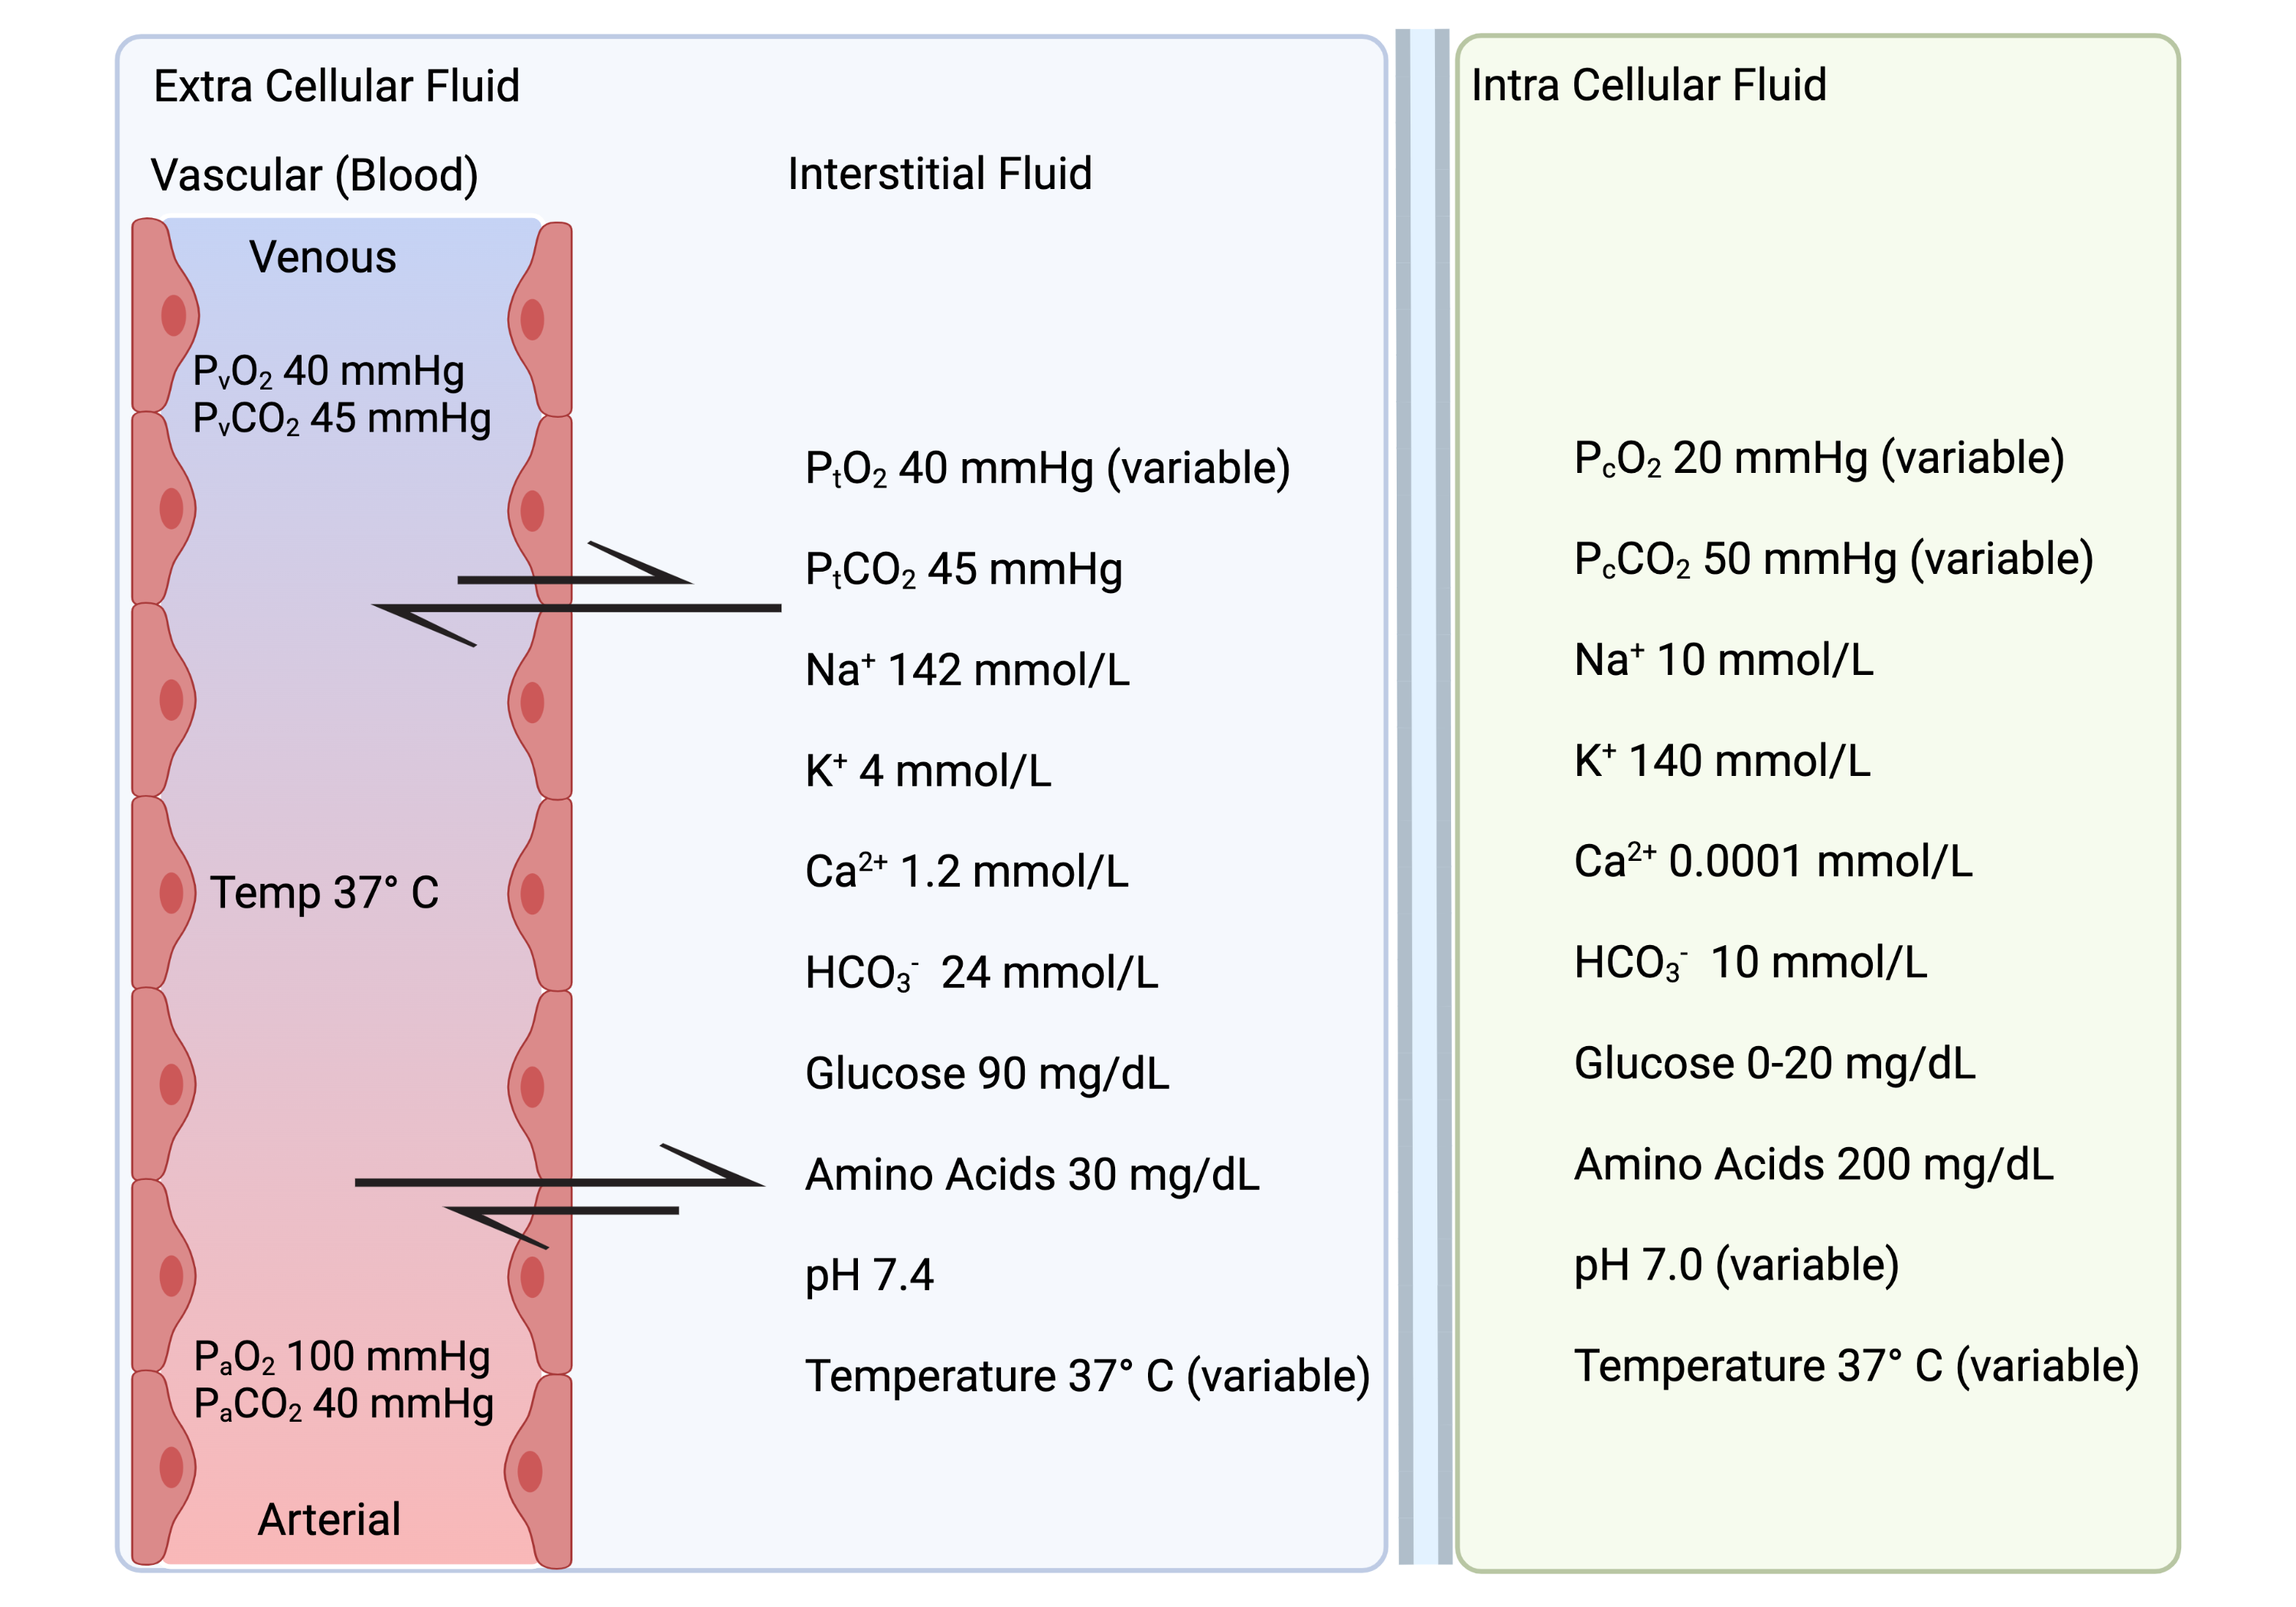
\includegraphics[width=1.0\linewidth]{./figure/ecf.png}
    \caption{Extra-cellular (Vascular \& Interstitial) and Intra-cellular Fluid \footnotesize{(Created with BioRender.com)}}
    \label{fig:ecf_respiration}
\end{figure}


\subsection{Factors Influencing Diffusion}

The factors influencing diffusion are provided in the following equation:
\vspace{4 mm}
\begin{equation}
    \dot{D} = \frac{A}{T} \times d \times (P_1 - P_2)
    \label{diffusion}
\end{equation}
\vspace{4mm}

\begin{itemize}
    \item $\dot{D}$ is diffusion as a rate (amount of substances over time)
    \item A is the surface area that diffusion can occur
    \item T is the thickness of the membrane through which diffusion can occur
    \item d is a diffusion coefficient that is related to the solubility and molecular weight of the substance diffusing
    \item $P_1 - P_2$ is the partial pressure gradient
\end{itemize}

Equation \ref{diffusion} assumes that the membrane is permeable to the substance being diffused. Which means there are no membrane restrictions to diffusion other than the surface area or thickness in the equation. Since that is the situation for the diffusion of $O_2$ and $CO_2$ across the cell membrane, capillary membrane and alveolar-capillary membrane this assumption is appropriate for respiration.\footnotemark\footnotetext{Note, if the membrane was only semi-permeable to $O_2$ and $CO_2$ then this equation then to model the situation more accurately the equation would need a permeability coefficient, as we have seen for filtration across the capillary.}

\subsubsection{Diffusion of $O_2$ and $CO_2$}

Since a nearly equal amount of $O_2$ and $CO_2$ is diffused across the cell, capillary and alveolar-capillary membrane during the microcirculation of blood the diffusion rates are, for all intents and purposes, equal under physiological conditions. They are always crossing the same membranes and therefore have the same $A$ and $T$. Since, as can be seen in Figure \ref{fig:ecf_respiration} the partial pressure gradients ($P_1 - P_2$) are not equal, the diffusion coefficient ($d$) must be (and indeed) is different between $O_2$ and $CO_2$. As can be deduced from Equation \ref{diffusion}, and the fact that $CO_2$ has a lower partial pressure gradient, $CO_2$ has a higher $d$ due to a higher solubility.\footnotemark\footnotetext{This relationship between solubility, partial pressure and diffusion is much more complicated than this since not only does solubility influence the diffusion coefficient and the rate of diffusion for a given partial pressure gradient, but solubility is inversely proportional to the partial pressure of the substance that is soluble based on Henry's law. These factors are beyond the depth of this text \cite{christmas_equations_2017}.}

\subsection{Tissue \& Cellular $O_2$ Uptake}

The diffusion of $O_2$ into the tissue (interstitial space) reduces the partial pressure of $O_2$ in the blood (See Figure \ref{fig:tissue_diffusion}). The $PO_2$ at the venous end of the capillary is the $P_vO_2$ and reflects how much $O_2$ has been taken in by the cells. An important concept is that the $P_vO_2$ from different areas of the body can be quite different. The regional $P_vO_2$ depends on the regional metabolism. While the $P_aO_2$ is the same throughout the arterial circulation, the $P_vO_2$ is different throughout the venous circulation, but continues to mix and become similar until the final mixing chambers of the right atrium and ventricles are reached. In other words, the $P_vO_2$ in the right ventricle represents a weighted mean from the entire body. And it is the $P_vO_2$ from the right ventricle that gets sent to the lungs, which means all of the alveoli receiving blood get blood with the same $PO_2$. Under resting conditions approximately 5 $mL O_2 / 100 mL$ of blood is taken in by tissues \cite{hall_guyton_2020}. However, this is an average and the true value is variable across the body with tissues such as the heart, brain and breathing skeletal muscles being slightly higher at rest, and inactive skeletal muscle lower when at rest (per unit volume).

\begin{figure}[!h]
    \centering
    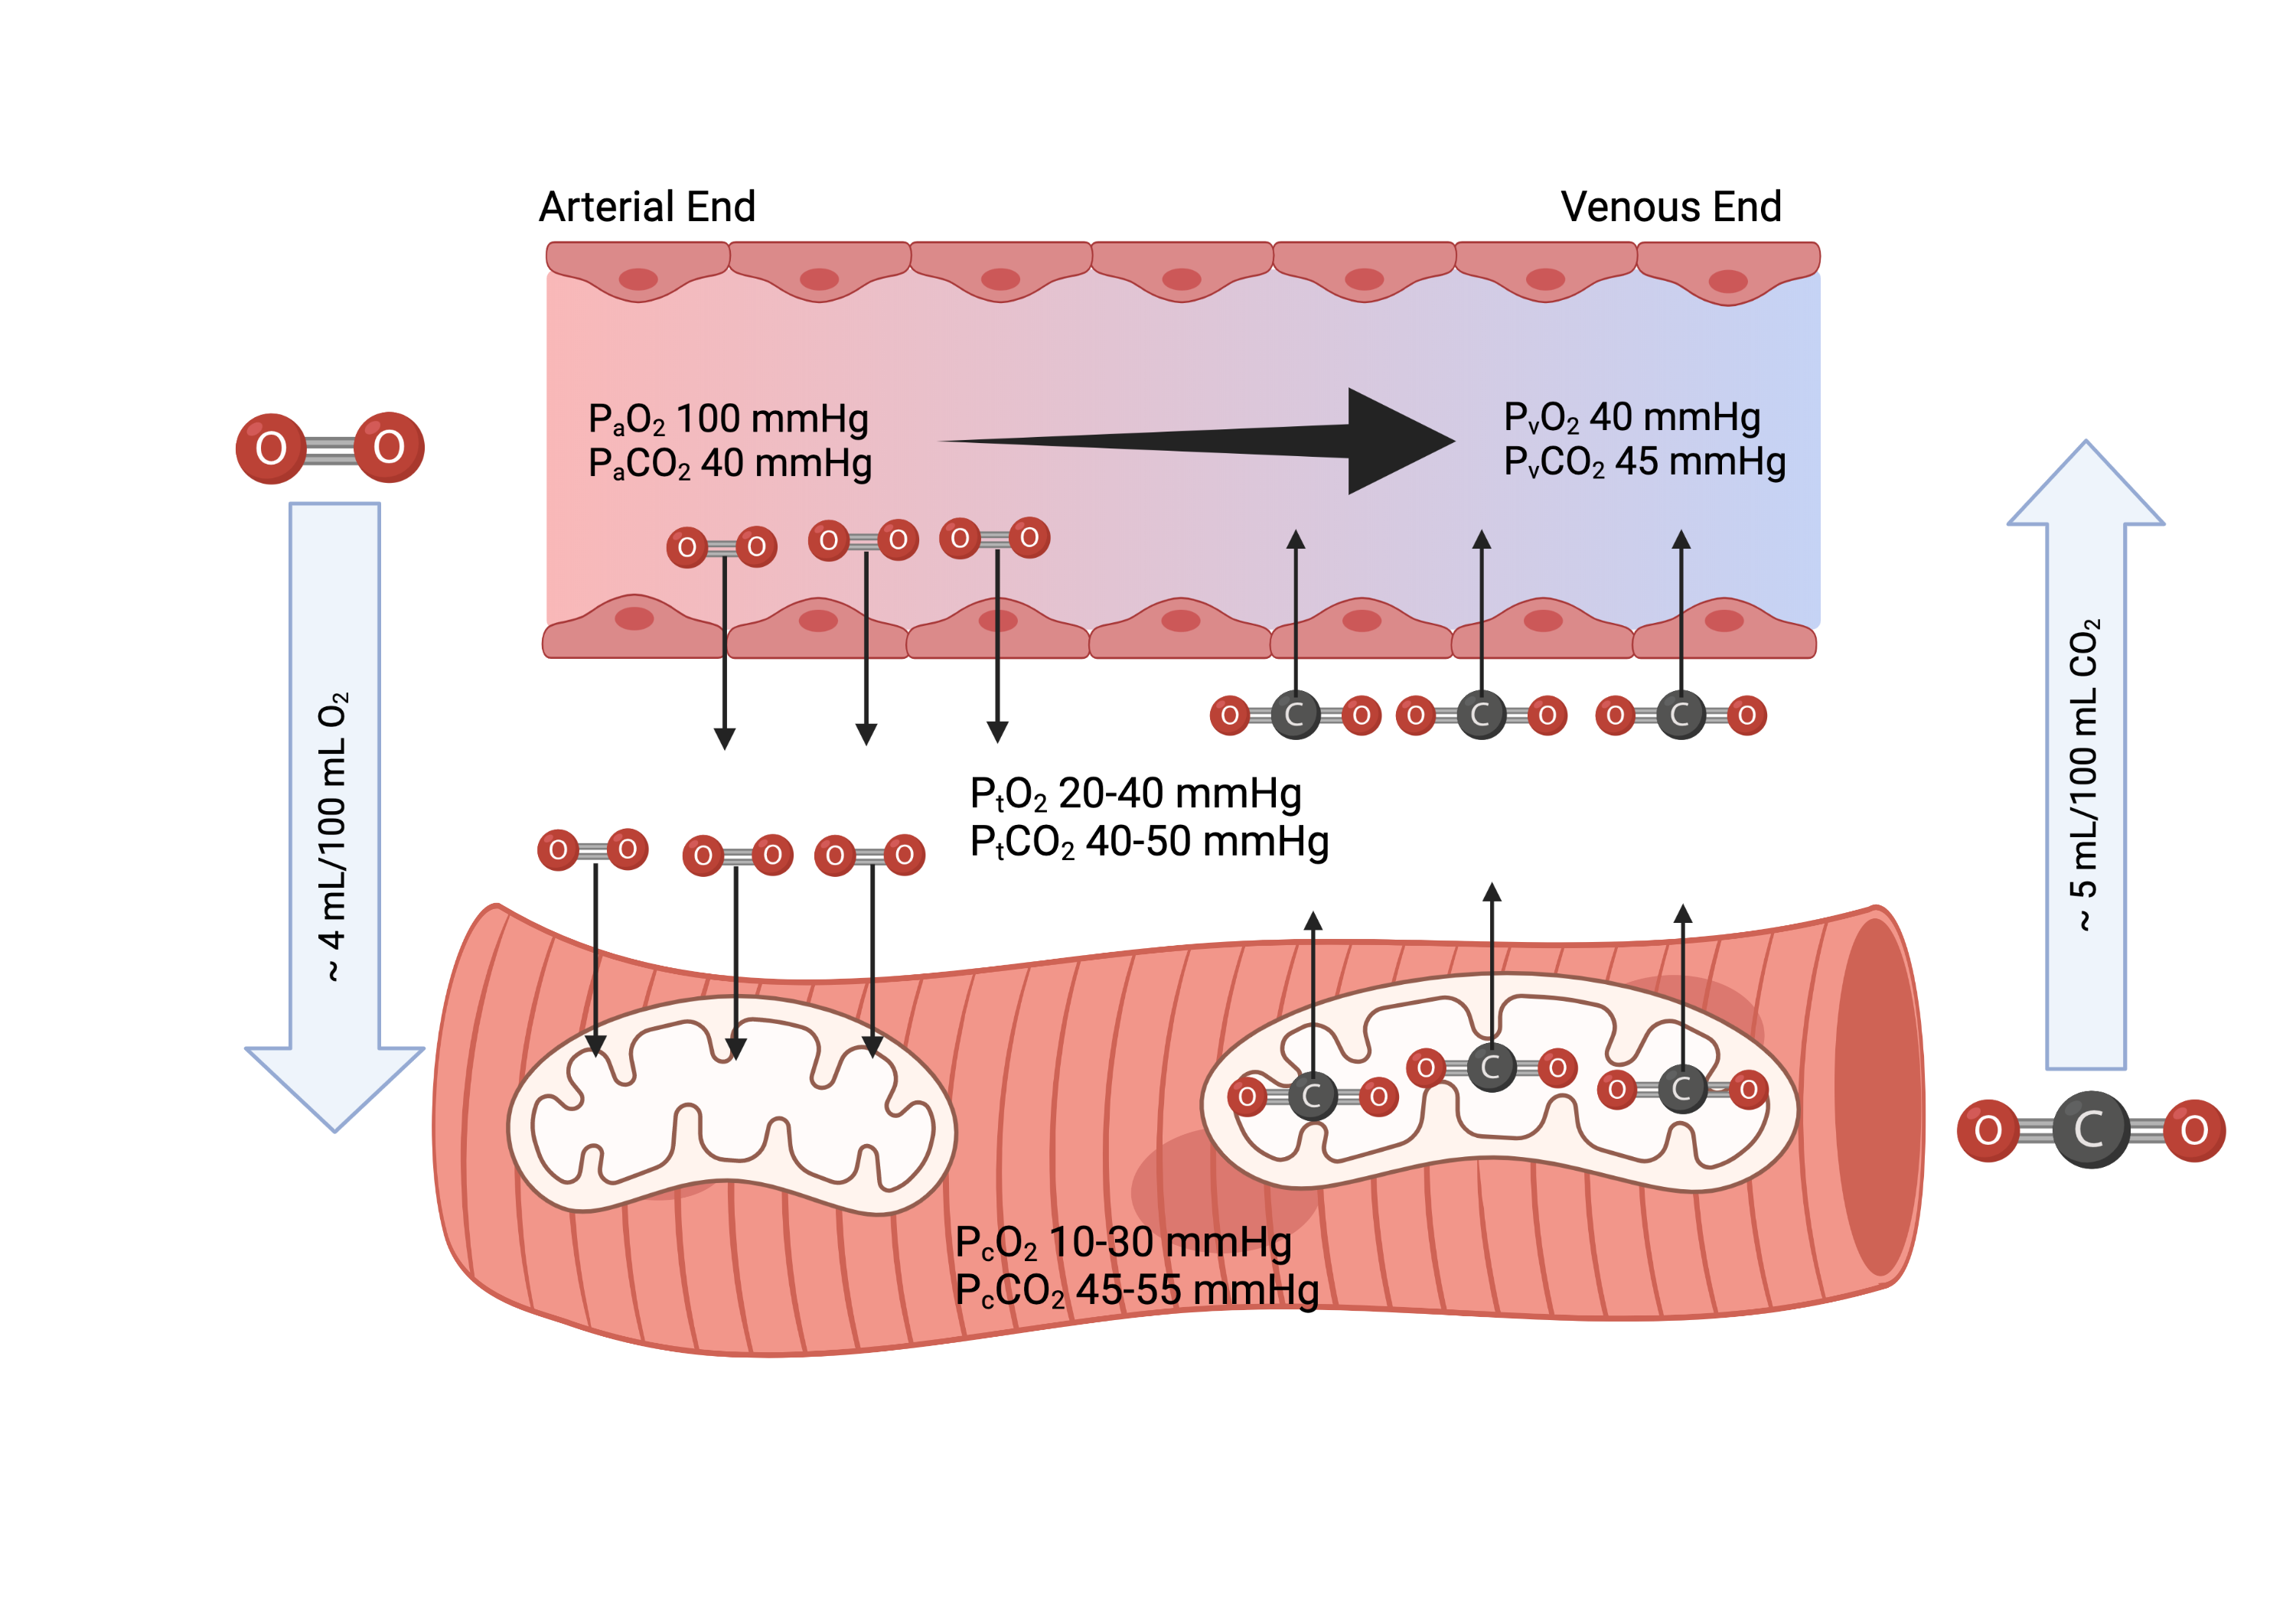
\includegraphics[width=1.0\linewidth]{./figure/tissue_diffusion.png}
    \caption{Tissue Diffusion of $O_2$ \& $CO_2$ \footnotesize{(Created with BioRender.com)}}
    \label{fig:tissue_diffusion}
\end{figure}

\subsubsection{Effect of Cellular Respiration}

There is a linear relationship between tissue metabolism, cellular respiration and $O_2$ utilization. Since the rate of the energetic pathways is related to the ATP:ADP ratio (normally 5:1), alterations to the amount of ADP in a cell tend to result in proportional changes to the rate of $O_2$ utilization. For example, if cellular ADP is $\frac{1}{2}$ of its normal value then $O_2$ utilization will be $\frac{1}{2}$ its normal value (ATP:ADP ratio might be 11:1). If cellular ADP is $1.5 \times$ higher than normal, then $O_2$ utilization is $1.5 \times$ higher than normal (ATP:ADP ratio might be 3:1) \cite{hall_guyton_2020}. The take home message is that the rate of $O_2$ utilization in the energetic pathways determines the rate of uptake of $O_2$ by the tissues and cells, and the venous $O_2$. 

\subsubsection{Myoglobin}

Myoglobin was introduced in Chapter \ref{chp:energetics} on Energetics and highlighted as a fundamental difference between SO, FOG and FG muscle fibers (Table \ref{table:Muscle_Fiber_Energetics}). SO muscle fibers express (synthesize and contain) more myoglobin. Myoglobin is a protein in the same family as hemoglobin. It is capable of binding $O_2$ molecules, which removes them from solution and thus lowers the $P_cO_2$ so which encourages more diffusion by maintaining the partial pressure gradient. The binding affinity of myoglobin for $O_2$ is based on the $P_cO_2$ with the myoglobin-$O_2$ dissociation curve (See Figure \ref{fig:myoglobin_dissociation}).


\begin{figure}[!h]
    \centering
    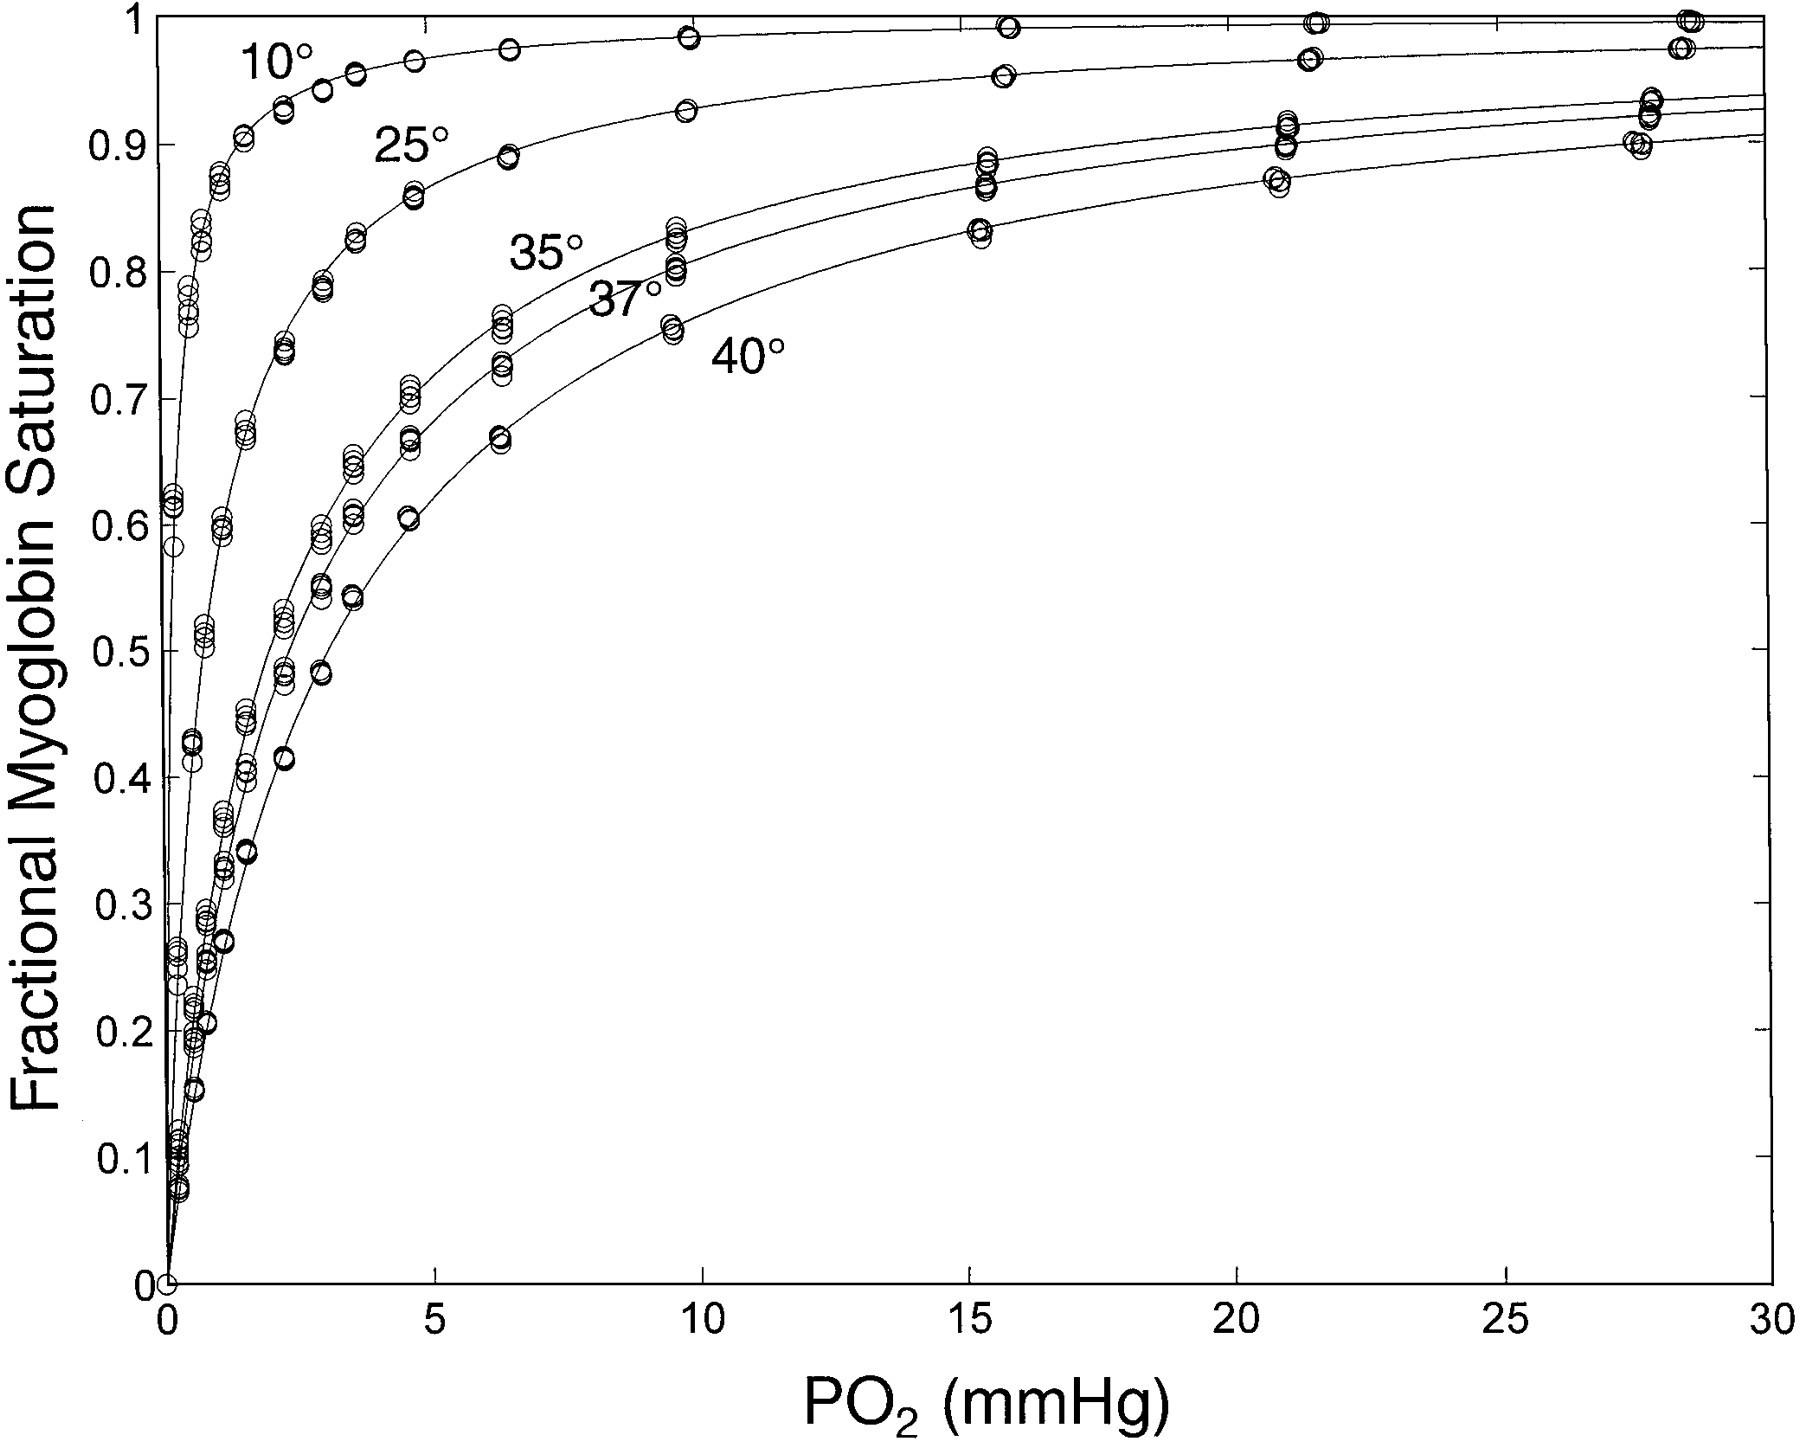
\includegraphics[width = 1.0\linewidth]{./figure/myoglobin_dissociation.jpeg}
    \caption{Myoglobin-$O_2$ dissociation curve as a function of temperature at a pH of 7.0 \footnotesize{(From \cite{schenkman_myoglobin_1997})}}
    \label{fig:myoglobin_dissociation}
\end{figure}

As $O_2$ utilization increases in a muscle fiber the $P_cO_2$ will drop which encourages dissociation (release) of $O_2$ from myoglobin and discourages $O_2$ entering the muscle from binding to myoglobin. With increased temperature ($40^{\circ} C$) the curve shifts right which encourages additional dissociation (release) of $O_2$ from myoglobin. Not depicted in Figure \ref{fig:myoglobin} is an additional rightward shift of the curve if pH drops below the normal resting muscle fiber value of 7.0. The rightward shifts of the myoglobin-$O_2$ dissociation curve in a muscle fiber encourage the release of $O_2$. These rightward shifts (increased temperature and decreased pH) are associated with increased metabolism, which is precisely when the fiber needs myoglobin to release its storage of $O_2$ for diffusion into the mitochondria. At rest (normal temperature and pH) the leftward shift encourages more myoglobin to bind $O_2$. Even lower than normal body temperature (normal body temperature is $37^{\circ} C$), encourages additional storage. It's important to note that regardless of these shifts, with a low enough $P_cO_2$, myoglobin releases $O_2$, and with a high enough $P_cO_2$, myoglobin binds and therefore stores $O_2$.

%Expand on myoglobin's role in breath holding? Aerobic capacity? As an adaptation?

\subsection{Tissue $CO_2$ Release}
Partial pressure driven diffusion of $CO_2$ follows the same reasoning as with the diffusion of $O_2$ but in the opposite direction (See Figure \ref{fig:tissue_diffusion}). The cellular partial pressure of $CO_2$ ($P_cCO_2$) is the highest partial pressure which drives diffusion of $CO_2$ out of the cell into the interstitial fluid. The $P_tCO_2$ is higher than the $Pa_CO_2$ in the arterial blood at the arterial end of the capillary, which drives $CO_2$ into the capillary. The $P_cCO_2$ is variable based on the rate of $CO_2$ produced during aerobic metabolism (TCA). The diffusion of $CO_2$ into the blood increases the $PCO_2$ in blood flowing through the capillary. At the venous end the $P_vCO_2$ equilibrates to whatever is in the tissue which is higher than the $P_aCO_2$. There tends be wider fluctuation in $P_aCO_2$ than in $P_aO_2$ due to the much lower atmospheric partial pressure of $CO_2$. For reasons that will be partially elucidated in this chapter and more fully explained in Chapter \ref{chp:alveolar_oxygen} on Ventilation, variation in ventilation (breathing rate and volume) can create large fluctuations in $P_aCO_2$ with relatively little change in $P_aO_2$. Under resting conditions approximately 4 $mL CO_2 / 100 mL$ of blood is released from the tissues. 

\subsection{Respiratory Exchange Ratio (RER)}

The RER, introduced in Chapter \ref{chp:energetics} on Energetics, is based on the volume of $CO_2$ produced and released into the blood (and eventually expired by breathing); and the volume of $O_2$ taken in from the blood and utilized in the mitochondria. 
\begin{equation}
    RER = \frac{\dot{V}CO_2}{\dot{V}O_2}
\end{equation}
With a mixed substrate diet (fats and carbohydrates) the RER = 0.8, which is based at a cellular level on the release of approximately 4 $mL CO_2 / 100 mL$ and the uptake of approximately 5 $mL O_2 / 100 mL$. With a purely carbohydrate metabolism the RER = 1.0 and with purely fats it is $\approx$ 0.7. 

% Consider expanding the chemical explanation of why the ratio changes and relate to diets....


\section{Blood Transport}

Whether discussing venous blood (from tissues and cells to the lungs), or arterial blood (from the lungs to the tissues and cells), $O_2$ and $CO_2$ are being transported in the blood. The transport of $O_2$ and $CO_2$ in the blood has overlap (shared mechanisms) albeit with different proportions per mechanism. Overall, $CO_2$ has an additional transport option that is responsible for a large proportion of $CO_2$ transport.

A small amount of $O_2$ (approximately 1-2\%) and $CO_2$ (approximately 7\%) is transported simply as $O_2$ and $CO_2$ dissolved in the blood. This portion contributes to the partial pressures and therefore has a large role in diffusion and as a factor in determining the amount being carried in the blood. But it is clearly not the largest quantity of either $O_2$ or $CO_2$ being transported.

\subsection{Red Blood Cells}

Red blood cells (RBCs), also referred to as erythrocytes, constitute approximately 45\% of the total blood volume (Hematocrit, HcT). RBCs do not have a nucleus and therefore do not divide. They are regenerated and replaced regularly in the bone marrow through the process called erythropoiesis. Erythropoiesis is stimulated by the hormone erythropoietin (EPO) which is released from the kidneys.

\begin{figure}[!h]
    \centering
    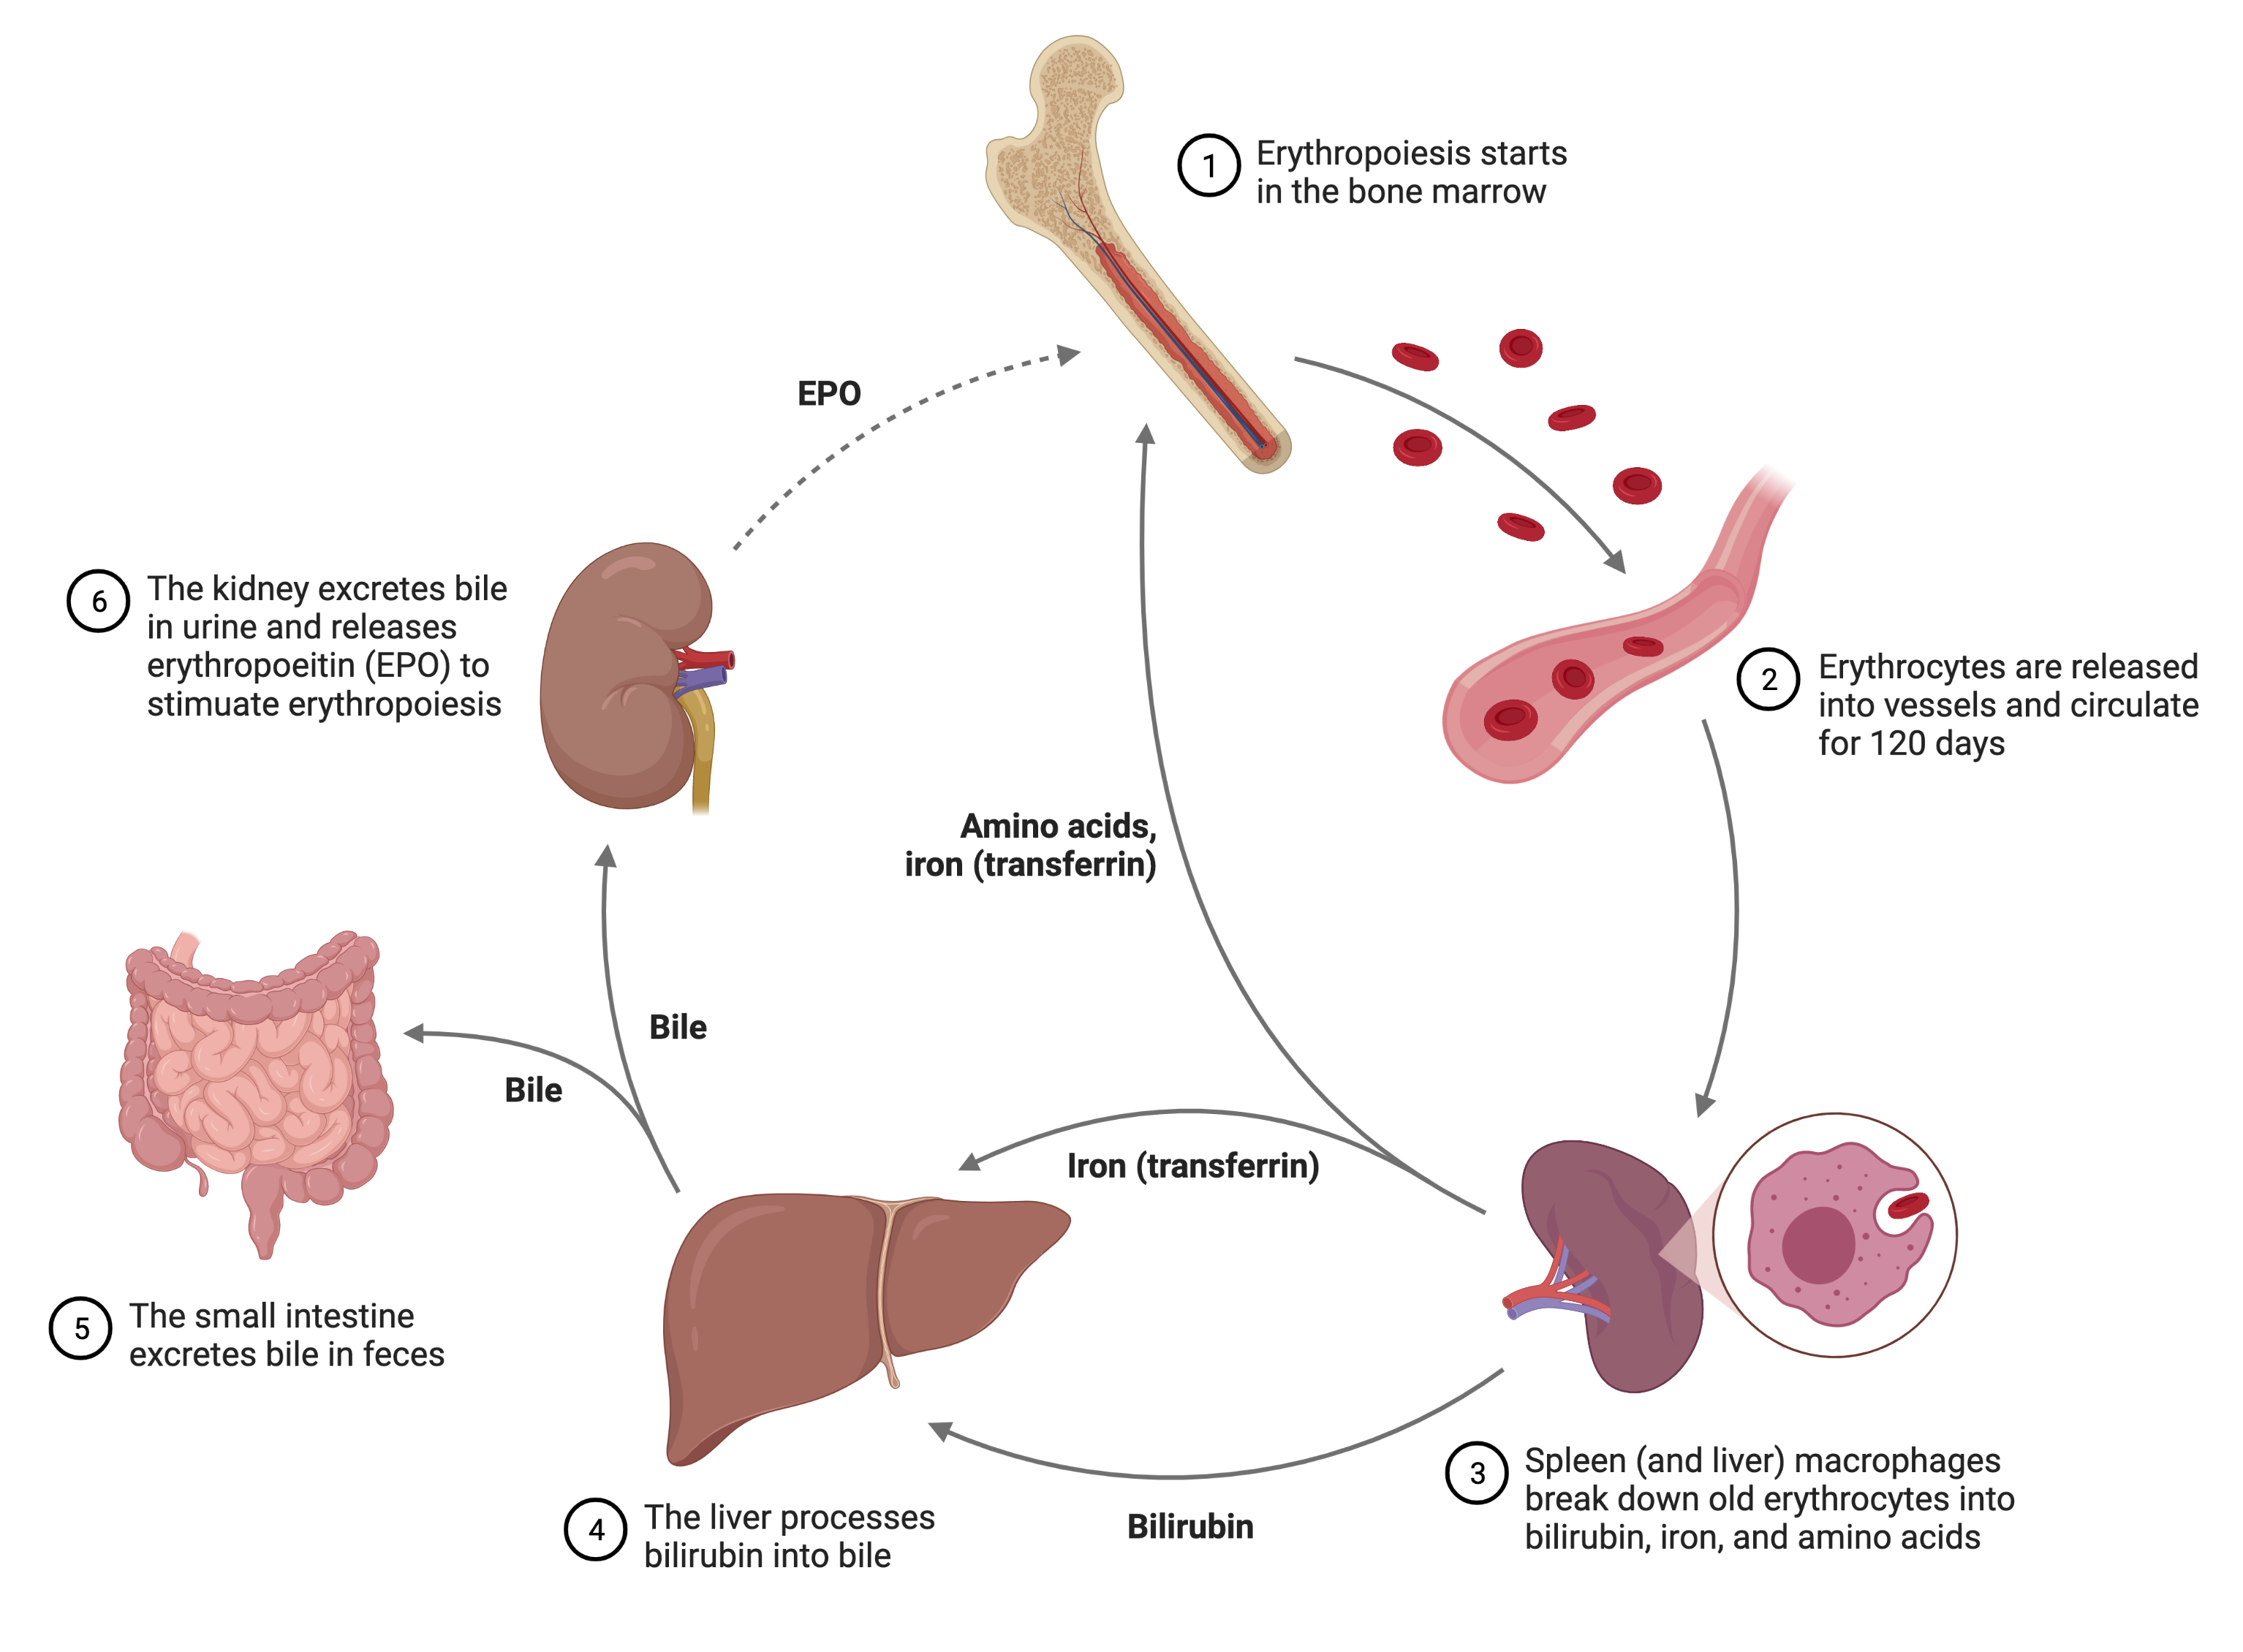
\includegraphics[width=1.0\linewidth]{./figure/RBC.png}
    \caption{Life Cycle of Erythrocytes \footnotesize{(Created with RioRender)}}
    \label{fig:RBC}
\end{figure}

EPO is secreted by the kidneys at a regular rate, possibly in response to bile filtration, to compensate for normal cellular turnover (See Figure \ref{fig:RBC}). EPO release increases in response to cellular hypoxia and stimulates additional erythropoiesis as a compensatory mechanism in an attempt to solve the problem of cellular hypoxia. Common causes of cellular hypoxia resulting in elevated levels of EPO include altitude or low barometric pressure (hypobaric) exposure which reduce environmental and therefore arterial $PO_2$; anemia (reduced RBCs), and hypoxemia due to chronic lung disease. RBCs contain hemoglobin (HgB). 

Hgb is an iron-containing oxygen-transport protein. While HcT is the percent of blood that is composed of RBCs, HgB is the number of grams per liter of HgB in blood (usually per deciliter or 100 milliliter\footnotemark\footnotetext{1 $dL$ is equal to 100 $mL$}). A normal HgB level is approximately 15 $g/dL$ with a range 12 to 20 $g/dL$.

HgB has an $O_2$-binding capacity of 1.34 $mL O_2 / g$ which increases the total blood oxygen capacity seventy-fold compared to dissolved oxygen in blood. A HgB molecule can carry up to four oxygen molecules. When fully saturated with $O_2$ and with a HgB of 15 $g/dL$, there is approximately ($15 \times 1.34 = 20.1 mL O_2/ 100 mL$ of blood. This estimate varies predictably and proportional to the amount of actual saturation and HgB.

%Anemia section
\paragraph{Anemia}
Anemia with HcT in the range of 0.3 - 0.4 is common following surgery and a cause of fatigue and reduced endurance that will recover in several days when kidneys are healthy due to an increase in EPO release and associated erythropoiesis (or sooner if facilitated by a blood, or RBC, transfusion). Causes of anemia that are not reversible, and that continue until anemia progresses until HcT is less than 0.1, can result in death. Anemia is a, but not the only, cause of hypoxemia. With anemia, there is reduced oxygen carrying capacity in the blood. Chronic renal conditions, including chronic conditions such as heart failure that cause chronic renal insufficiency, will often result in anemia. When this occurs treatment can include the medication Epoetin alfa (Epogen, Procrit) which is a human made form of erythrpoeitin that stimulates RBC production in the bone marrow.

% Consider expanding anemia section

\paragraph{Transfusions \& ABO Blood Types}

RBCs can have A and/or B antigens on their cell membrane. Blood can occur with four possible types, A, B, AB or O (O being an indication that the RBC membrane has neither A or B antigens). Whatever antigen a RBC membrane has, it's plasma contains anti-bodies for the opposite antigen. If A antigen is present on the RBC then the plasma has Anti-B antibodies. If A and B antigen is present (AB blood) then the plasma has neither antibody. If no antigen is present (O blood) then the plasma has both antibodies. The type of blood influences whether the blood can be donated or received as summarized in Figure \ref{fig:ABO}.

\begin{figure}[!h]
    \centering
    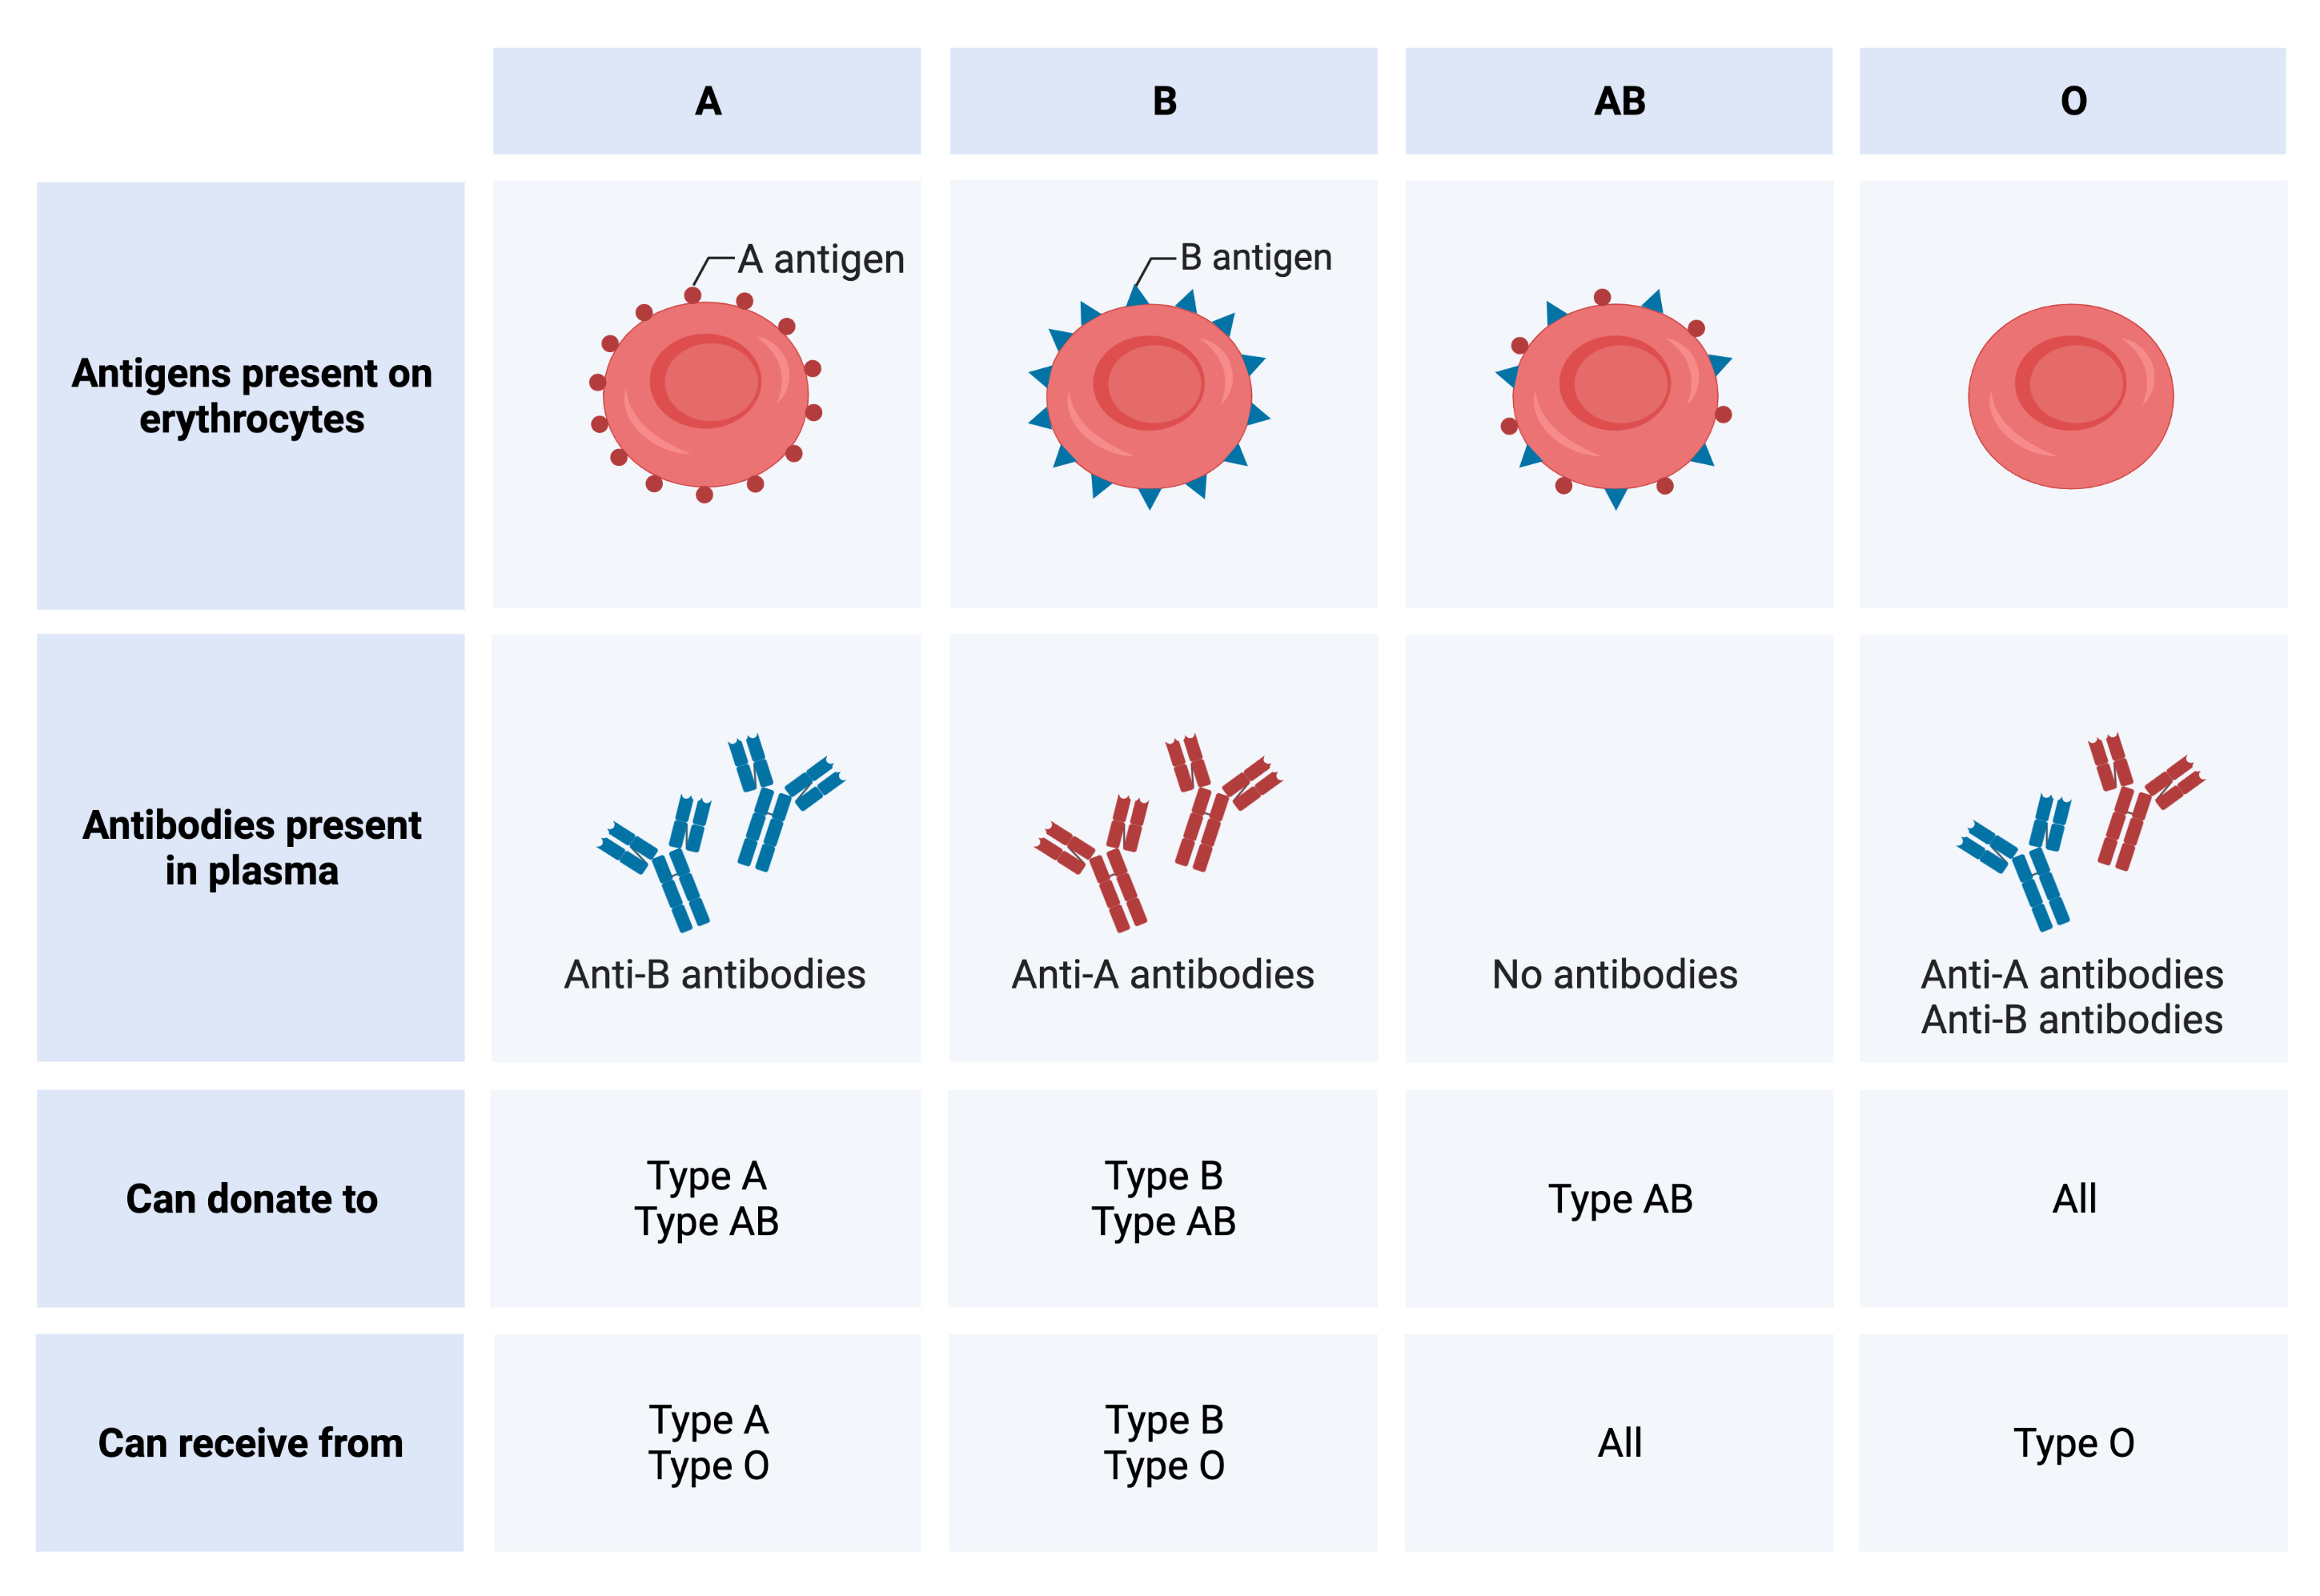
\includegraphics[width=1.0\linewidth]{./figure/ABO.png}
    \caption{ABO Blood Types \footnotesize{(Created with BioRender.com)}}
    \label{fig:ABO}
\end{figure}

\subsubsection{Blood Transport of $CO_2$}

There are three ways that $CO_2$ is transported in the blood (See Figure \ref{fig:co2_transport}). $CO_2$ is transported directly in the blood in a small quantity (7\%) which generates the partial pressure of $CO_2$ in the blood ($P_aCO_2$ in arterial blood, and $P_vCO_2$ in the venous blood). 

\begin{figure}[!h]
    \centering
    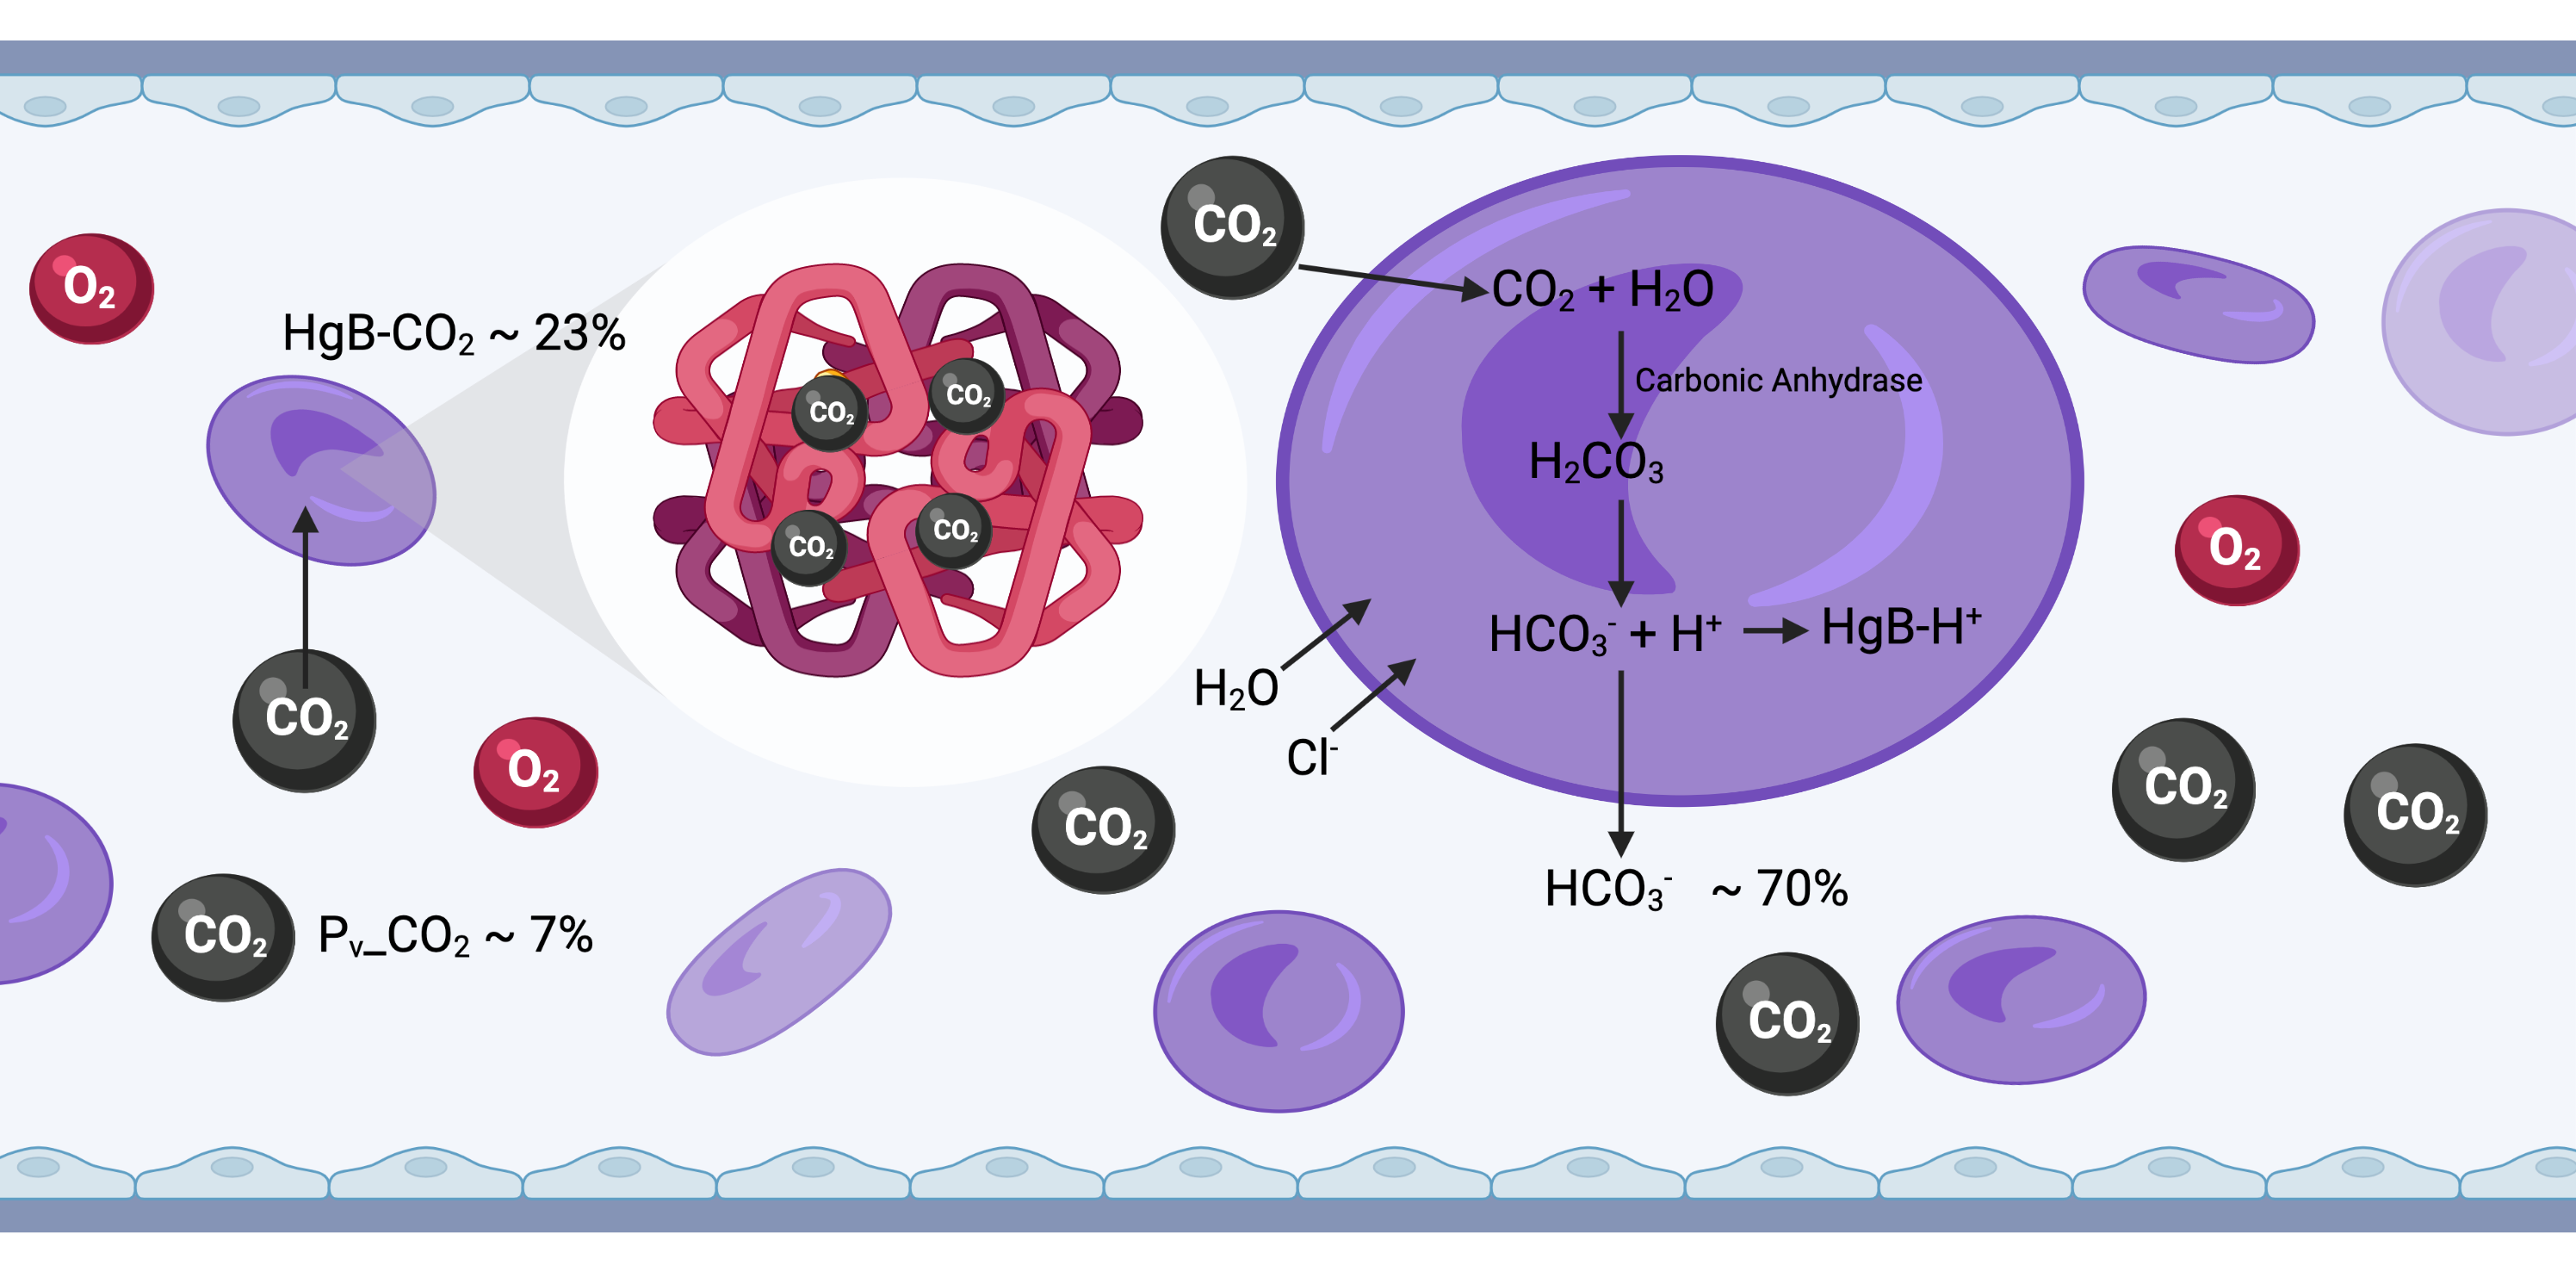
\includegraphics[width=1.0\linewidth]{./figure/co2_transport.png}
    \caption{Blood Transport of $CO_2$ \footnotesize{(Created with BioRender.com)}}
    \label{fig:co2_transport}
\end{figure}

The majority of $CO_2$ is transported as bicarbonate ($HCO_3^-$) (approximately 70\%) through the following chemical reaction within the red blood cells (RBCs). 
Within the RBC $CO_2 + H_2O \rightarrow H_2CO_3$ which is facilitated by the enzyme carbonic anhydrase. To buffer this acid, a hemoglobin (HgB) will bind with $H^+$ to form $HgB-H^+$ (which stays in the RBC) and a molecule of $HCO_3^-$ which is released into the plasma through an exchange with $Cl^-$ in a process known as the chloride shift.

The remaining $CO_2$ (approximately 23\%) binds directly with HgB to form $HgB-CO_2$ which is referred to as carbaminohemoglobin (not to be confused with carboxyhemoglobin which is $HgB-CO$ from the inhalation of carbon monoxide, the result being carbon monoxide poisoning). 

These processes are facilitated by the movement of $CO_2$ into the RBCs which occurs due to the $PCO_2$ gradient between the plasma and the RBC. As the above reactions proceed the RBC $PCO_2$ drops and $CO_2$ will diffuse into the RBCs until the $PCO_2$ in the plasma and the RBC are equalized. As a reminder, gradient that pushes $CO_2$ into the plasma and then the RBCs originates in the mitochondria where $CO_2$ is being generated.


\subsection{Blood Transport of $O_2$}

$O_2$ is transported directly in the blood in a small quantity (1-2\%) which generates the partial pressure of $O_2$ in the blood ($P_aO_2$ in arterial blood, and $P_vO_2$ in the venous blood). 

The majority of $O_2$ is transported in RBCs, attached to HgB. The partial pressure ($PO_2$) gradients facilitate the movement across membranes, including into the RBCs, which then allow $O_2$-HgB binding. The affinity for $O_2$-HgB binding is related to the $PO_2$ as well as to the number of binding sites of a HgB molecule already bound with $O_2$. With each binding site that has an $O_2$ bound to it, there is an increased affinity for the other binding sites to bind. The binding of $O_2$ to HgB is also influenced by the temperature (increased temperature reduces $O_2$-HgB affinity), and the pH (acidity reduces $O_2$-HgB affinity), as well as a 2,3-bisphosphoglycerate (BPG) (increased BPG reduces affinity). Of these factors that shift the curve, temperature and pH vary quickly based on body status (exercise vs. rest), and between parts of the body (working muscle vs. nonworking muscle; and between muscle and lungs). But BPG varies across longer time periods as a RBC adaptation. 
BPG is found in RBCs and preferentially binds to HgB when $O_2$ is not bound to HgB. If there is an increase in BPG there is reduced affinity of HgB to bind with $O_2$ so that oxygen unloads from HgB more quickly when $PO_2$ drops. At first this sounds negative. However, reducing the affinity of HgB for $O_2$ is helpful when the goal is to release $O_2$ so that it can diffuse into the metabolically active cells requiring $O_2$. Fluctuations in BPG tend to be RBC adaptations in response to chronic conditions such as chronic anemia, pulmonary disease and as an adaptation to high altitude.

The relationship between the $PO_2$ and the amount of $O_2$ bound to HgB expressed as the percentage of binding sites of HgB with $O_2$ (oxygen saturation, $SO_2$) is given in the oxyhemoglobin dissociation curve. The features of this curve depict, first, the relationship between $PO_2$ and $SO_2$; and shifts in the curve depict the influence of pH, $PCO_2$, temperature, and BPG. The curve is usually considered from the perspective of arterial blood and therefore the relationship between $P_aO_2$ and $S_aO_2$ and the diffusion of $O_2$ during loading of HgB with $O_2$. When considering $P_aO_2$ and $S_aO_2$ the oxygen content of arterial blood that is being delivered is being assessed, reduced values indicate hypoxemia. However, it is equally valid to consider the curve in the capillary or venous blood when considering the utilization of $O_2$ by the cells of the body; and the influence of the $O_2$-HgB affinity on releasing (unloading) $O_2$ into the tissues.
Note, when $S_aO_2$ is estimated with a pulsed oximeter it is abbreviated as $S_p_O_2$.

\subsubsection{Oxyhemoglogin Dissociation Curve}

Figure \ref{fig:oxyhemo1} depicts the oxyhemoglobin dissociation curve simulated with two different pH. The Y-axis is the $SO_2$ and the X-axis is the $PO_2$. The $PO_2$ is primary determinant $O_2$-HgB binding, and pH is a second determinant. The sigmoidal relationship identifies an important area in this relationship. A critical juncture where reductions of $PO_2 < 60$ include rapid reductions in $SO_2$ due to a reduced $O_2$-HgB binding affinity. When considering capillary and venous blood, this is a helpful attribute for unloading $O_2$ for diffusion into cells. However, if arterial $O_2$ partial pressure ($P_aO_2$) drops below 60 $mmHg$ then there is barely enough $O_2$-HgB binding (hypoxemia is a $P_aO_2 <60$ or $S_aO_2 < 90$). And further drops in $P_aO_2$ result in rapid and significant drops in $S_aO_2$. The implications of the sigmoidal shape of the curve is further discussed in Chapter \ref{chp:alveolar_oxygen} on Ventilation since the most common reason for drops in $P_aO_2$ are changes and insufficiency in ventilation. 

\begin{figure}[!h]
    \centering
    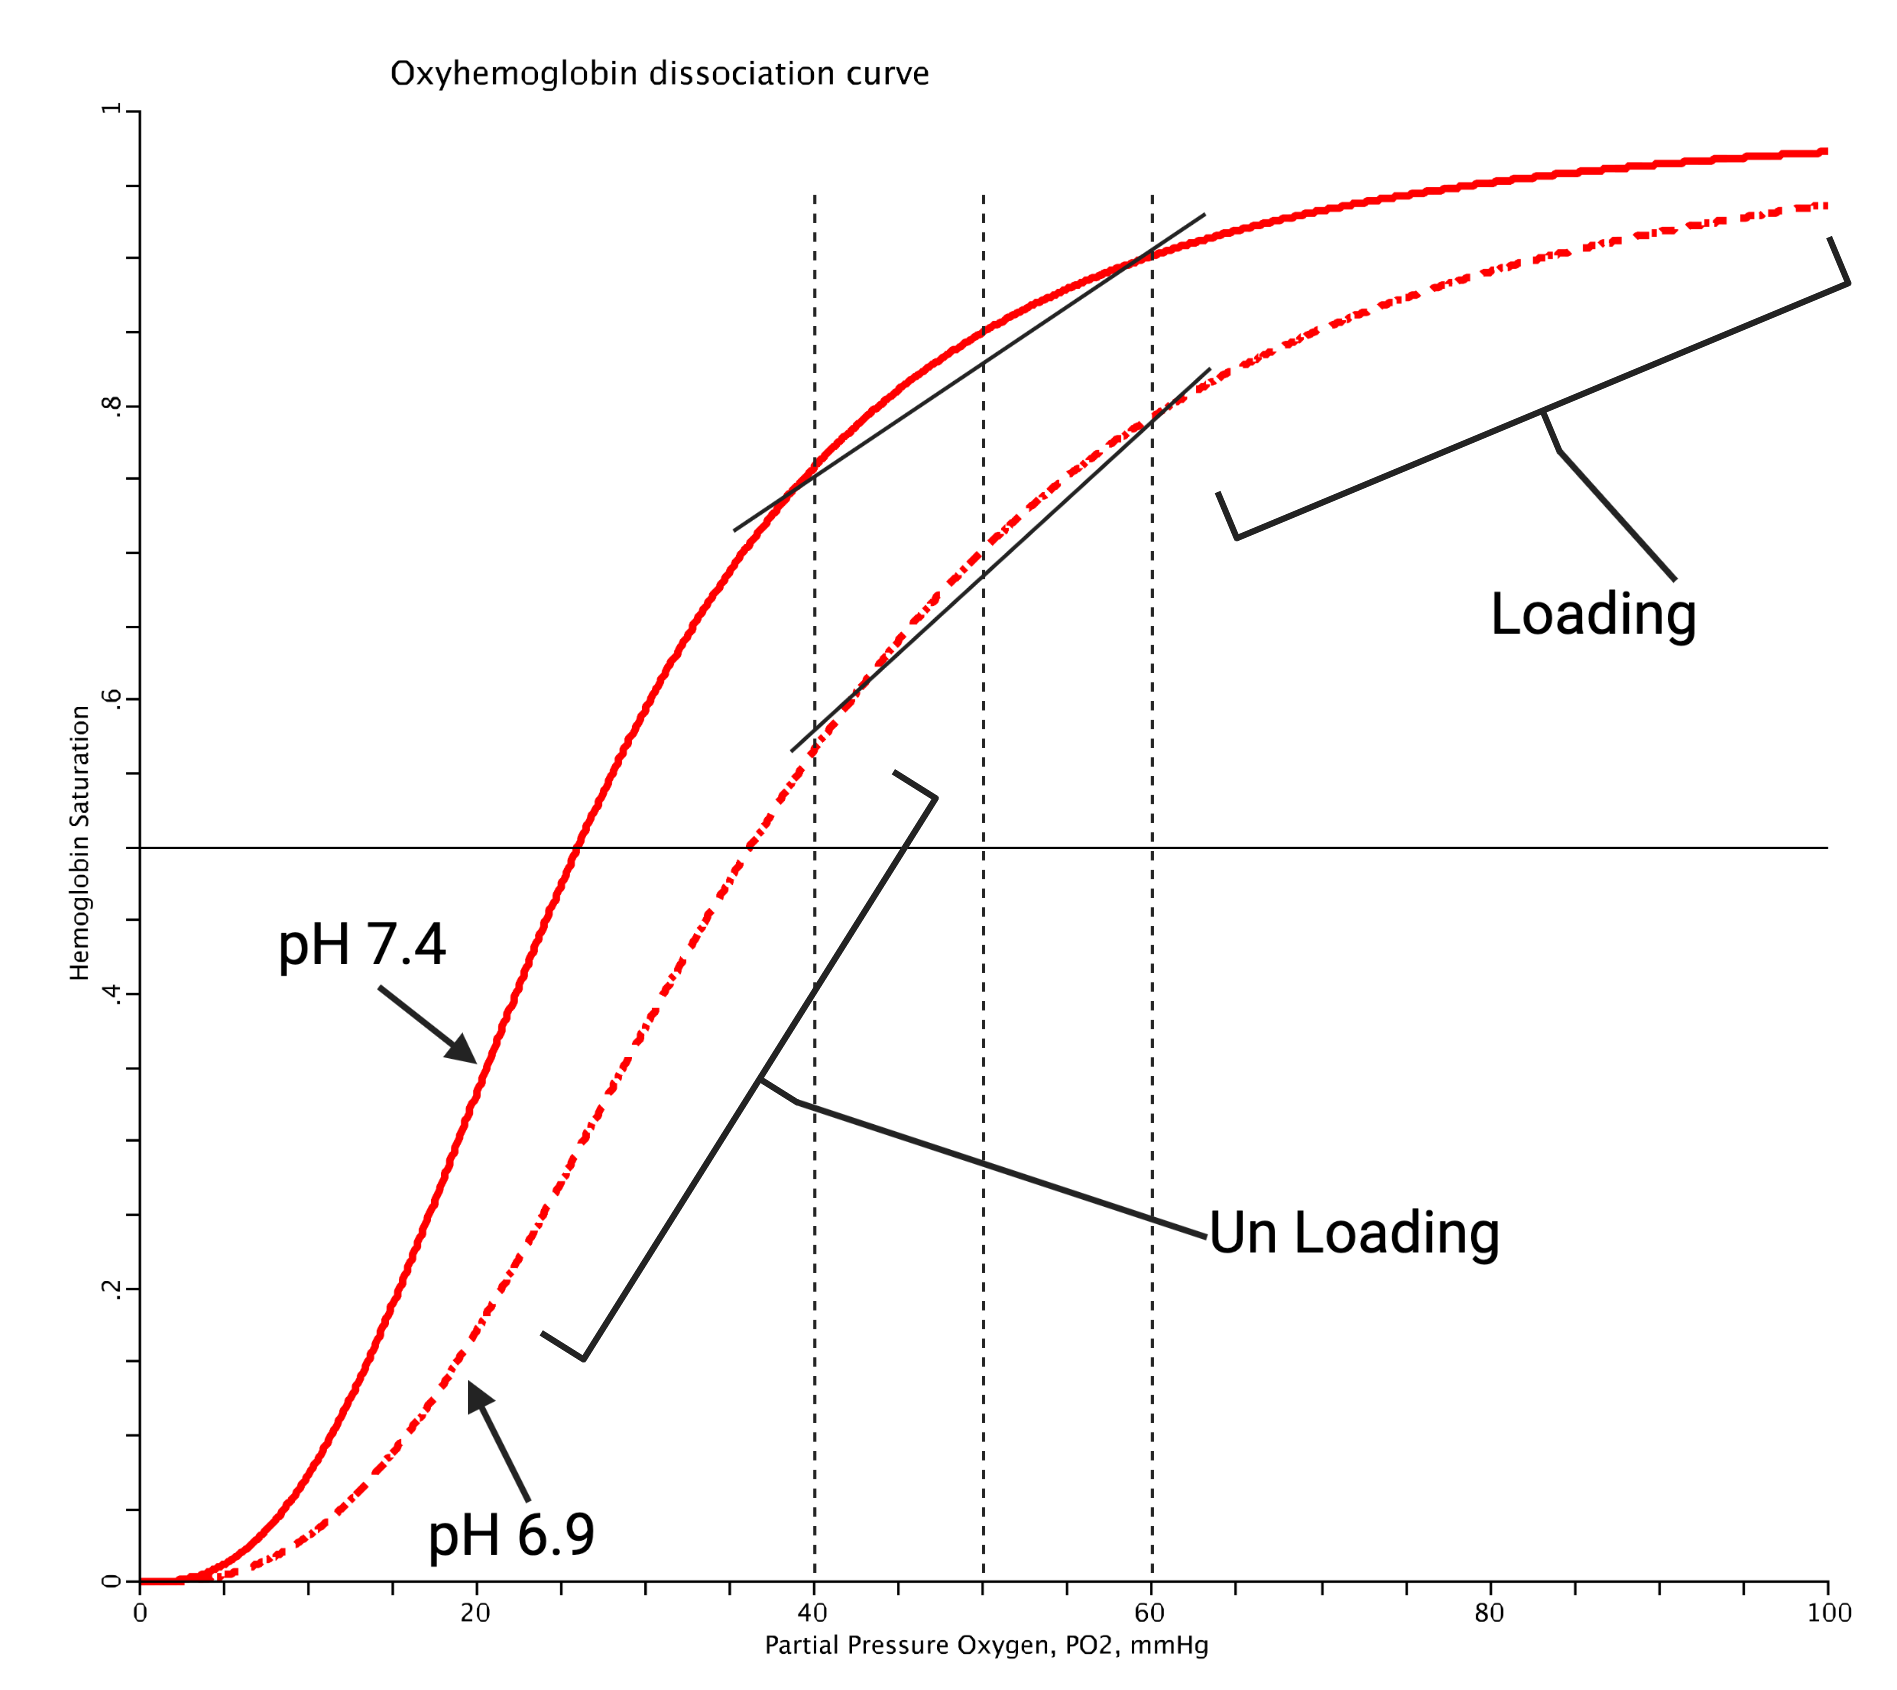
\includegraphics[width=1.0\linewidth]{./figure/oxyhemo1.png}
    \caption{Oxyhemoglobin Dissociation Curve \footnotesize{(Simulation performed with JSim\footnotemark\footnotetext{JSim is a simulation system created for physiological simulation under the Physiome project, \url{https://www.imagwiki.nibib.nih.gov/physiome/jsim}})}}
    \label{fig:oxyhemo1}
\end{figure}

Table \ref{table:oxyhemo} depicts a linear approximation at the critical juncture in the oxyhemoglobin curve that is worthwhile to remember in the interpretation of arterial blood gases (ABGs) or pulsed oximetry. If $S_pO_2$ is 90\%, then $P_aO_2$ can be estimated at 90 $mmHg$, and vice versa. A further drop in $P_aO_2$ of 10 $mmHg$ to 50 $mmHg$ will result in a drop in $S_pO_2$ to 80\%.

\begin{table}[h!]
\centering
\begin{tabular}{||c|c|c|c||} 
 \hline
 $S_aO_2$ & 70 & 80 & 90 \\ 
 \hline
 $P_aO_2$ & 40 & 50 & 60 \\[1ex] 
 \hline
\end{tabular}
\caption{Linear Approximation of Oxyhemoglobin Dissociation Curve}
\label{table:oxyhemo}
\end{table}

Figure \ref{fig:oxyhemo1} also depicts a right shift to the oxyhemoglobin dissociation curve based on pH. Besides $PO_2$, pH has the largest impact on HgB binding affinity. Fluctuations to pH occur as the blood circulates from working skeletal muscles to the lungs. In working skeletal muscle the pH tends to be lower due to the production of $H^+$ from the energetic pathways. The broken line in Figure \ref{fig:oxyhemo1} estimates the oxyhemoglobin dissociation curve in the skeletal muscle during exercise (favors unloading of $O_2$) when pH can drop to as low as 6.9. As can be seen in the figure, at any given $PO_2$, less HgB is bound to oxygen with a lower pH. In working muscle this is helpful because it means more $O_2$ will be released from HgB and available for diffusion.


\section{Pulmonary Circulation}

The majority of pulmonary circulation is to the alveoli (small air sacs of the lung). Pulmonary (alveolar) circulation is a low pressure - high volume system with such a high density of capillaries that the blood flows almost as sheets in close contact surrounding the alveoli. Blood leaving the right ventricle (RV) flows into pulmonary arteries (venous blood) and into the alveolar circulation for respiration (gas exchange) with the alveoli to become arterial blood. After flowing through the capillaries of the alveoli this arterial blood returns to the left atrium (LA) through the pulmonary veins. 
Approximately 1-2\% of cardiac output is sent to the bronchial arteries of the lungs for oxygenation of lung cells. This circulation is from the systemic circulation (from the left ventricle), but it returns its venous blood to the heart through the pulmonary veins into the LA. This small amount of venous blood mixes with the otherwise arterial blood in the LA and has a minor, inconsequential, effect on the $P_aO_2$ and $S_aO_2$.

\paragraph{Pulmonary Circulation Pressures}

Pulmonary artery pressure (PAP) is synonymous with arterial blood pressure (BP) and has both systolic and diastolic components. PAP is much lower than BP under normal circumstances, approximately 15-30 $mmHg$ / 5-10 $mmHg$ with pulmonary capillary pressures approximately 7 $mmHg$. Central pulmonary venous pressure is the pressure in the LA, approximately 0-2 $mmHg$, which is similar to the central systemic venous pressure in the RA. 

Intensive (critical) care unit (ICU) monitoring for patients with cardiac or other blood flow or volume conditions are often monitored with a cathether that records pressure in the pulmonary artery for continuous PAP monitoring that can occasionally be pushed further into the pulmonary circulation to estimate the pulmonary capillary pressure with a measurement referred to as the pulmonary capillary wedge pressure (PCWP). The PAP and PCWP are utilized to assess whether left sided heart function is adequate for the current blood volume, or whether the pulmonary circulation pressures are rising. If the pulmonary circulation pressures are too high then the pulmonary microcirculation favors filtration which could result in pulmonary edema or effusion.

\paragraph{Pulmonary Microcirculation \& Lymphatics}

The same four pressures determine the microcirculation in the lungs as in peripheral capillaries and tissues with a few important differences. The pulmonary capillary hydrostatic pressure is lower and the interstitial fluid pressure is negative due to the loss of fluid through the alveolar membrane and resultant evaporation (incidental water loss through breathing). Alveolar capillary permeability is high, allowing extra amounts of protein to leak from the capillaries; therefore, interstitial fluid osmotic pressure is high. The alveolar walls are thin but are generally impermeable to the proteins and solute (but are permeable to water). Total microcirculation outward pressure moving out of the capillaries exceeds the inward pressure by about 1 $mmHg$ promoting a small continual loss of fluid from the pulmonary capillaries. The capillary fluid loss is removed from the area partly through lymphatic flow and partly through alveolar evaporation of water. Some of the fluid seeps through the lung interstitial tissue and ends up in the pleural cavity surrounding the lungs, where it is typically drained into the lymphatics that drain the pleural space.

The same safety factors exist to prevent edema as in the peripheral tissue, and the same factors can cause edema. An important difference between peripheral tissue edema and pulmonary tissue edema is that pulmonary tissue edema will become pulmonary edema (as in alveolar edema). Pulmonary (alveolar) edema is life threatening because it impairs pulmonary respiration and can cause hypoxemia. The most common cause of pulmonary edema is left sided heart failure. 

If there is a slow accumulation (more often caused by reduced vascular osmotic pressure, or poor lymph function) of pulmonary tissue edema it may cross the pleural membranes and result in pleural edema (commonly referred to as a pleural effusion). The most common causes of pleural effusion include: blockage of lymphatic drainage from the pleural cavity; heart failure causes excessively high peripheral and pulmonary capillary pressures;  decreased vascular osmotic pressure; increased capillary permeability caused by infection or any other source of inflammation of the pleural surfaces.

\paragraph{Regulation of Pulmonary Circulation}

The volume and rate of pulmonary circulation equals the volume and rate of systemic circulation. The venous return that enters the right side of the heart and flows to the pulmonary circulation must equal the output of the left ventricle. This equality does not have to be beat to beat, but certainly must be equal when integrated over time (i.e., minute by minute). Otherwise there would be an accumulation of blood in the pulmonary circulation that impairs blood flow, ventilation and respiration, if more entered the lungs than was ejected from the LV. Or, a continuous decrease in LV output, if more was ejected from the LV than came through the pulmonary circulation. Therefore, the overall regulation of pulmonary circulation (volume and rate) includes the same processes that regulate systemic circulation as covered in Chapter \ref{chp:blood_flow} and \ref{chp:blood_content}

As with the peripheral circulation the distribution of pulmonary circulation is largely dependent on local regulation. One fundamental difference is that local regulation of pulmonary (alveolar) circulation through tone (vaso dilation and constriction) of arterioles is opposite of muscular arterioles. In the muscular (systemic circulation) arterioles local indications of low $O_2$ concentration and high metabolism result in vasodilation in an effort to increase blood flow to those capillaries. However, in the pulmonary circulation arterioles, low $O_2$ concentration results in arteriole vasoconstriction, in an effort to shift blood away from those capillaries. This makes complete sense for the distribution of circulation in the lungs, where the reason for blood to be delivered to capillaries surrounding alveoli is to obtain $O_2$, not to deliver $O_2$. If some alveoli have poor airflow and low $P_AO_2$ then it is better for less blood to circulate to that alveolar-capillary network. Arterioles of alveoli-capillary networks that have high $P_AO_2$ vasodilate, to promote circulation to those alveoli with more $O_2$.

Respiratory sinus arrhythmia (RSA) refers to the observation that in healthy individuals at rest there is cyclic variation in heart rate with the respiratory (breathing) frequency. With inhalation (inspiration) HR tends to go up a few beats per minute; with exhalation (expiration) HR tends to diminish a few beats per minute. The RSA is a dominant source of what is called high frequency heart rate variability (HRV) and is associated with parasympathetic nervous system activity (vagal cardiac tone). It has been hypothesized that RSA helps to maximize blood flow through the pulmonary circulation when alveoli have more ventilation as a feedforward (not feedback) system of control. This control is feedforward because the HR increases in response to the same trigger for inhalation, not in response to there being more oxygen in the lungs. There is evidence that RSA helps to maximize ventilation - perfusion matching at rest \cite{hayano_hypothesis_2003}.

Chapter \ref{chp:alveolar_oxygen} on Ventilation considers the concept of ventilation - perfusion $\dot{V}/\dot{Q}$ matching, the impact of body position on $\dot{V}/\dot{Q}$ matching zones, and the impact of $\dot{V}/\dot{Q}$ matching on the $P_AO_2-P_aO_2$ gradient, otherwise known as the A-a gradient.

\section{External (Alveolar) Respiration}

External (alveolar) respiration is gas exchange between the alveolar capillary blood and the alveoli. As with in the systemic capillaries and tissues diffusion occurs with the partial pressure gradients of $O_2$ and $CO_2$. Diffusion is influenced by the factors in Equation \ref{diffusion}. The structure of alveoli (thin membrane with a high surface area) and alveolar capillaries (dense network forming sheets in close contact with the thin alveolar membrane) are well equipped for rapid diffusion and full equilibration of $O_2$ and $CO_2$ both at rest and with higher rates of pulmonary circulation such as with high cardiac output during maximal exercise.


\subsection{Alveolar $O_2$ Diffusion}

A ventilated alveoli at sea level has a partial pressure of oxygen ($P_AO_2$) of approximately 104 $mmHg$. The atmosphere at sea level has a partial pressure of $O_2$ of approximately 159.5 mmHg. The $PO_2$ from the atmosphere to the arterial blood drops as it passes into the alveoli because air is humidified (some of the pressure is now due to water molecules); because $CO_2$ is being diffused into the alveoli (some of the pressure is due to $CO_2$); and because $O_2$ is being diffused out of the alveoli (there is a regular reduction in the concentration of $O_2$). Maintaining a $P_AO_2 \approx 104 mmHg$ requires continuous air exchange with the atmosphere (alveolar ventilation, $V_A$, the primary topic for the next Chapter \ref{chp:alveolar_oxygen} on Ventilation.

The full equilibration of blood at a single alveoli is depicted in Figure \ref{fig:alveolar_equilibration}. Note that the $P_aO_2 = P_AO_2$. This requires alveoli with normal membrane thickness and surface area in contact with capillaries, and normal capillary membranes. During equilibration of $O_2$ binding to HgB based on the $P_aO_2$ according to the oxyhemoglobin curve (Figure \ref{fig:oxyhemo1}) ensures the blood $O_2$ carrying capacity is sufficient to support cellular respiration. 

\begin{figure}[!h]
    \centering
    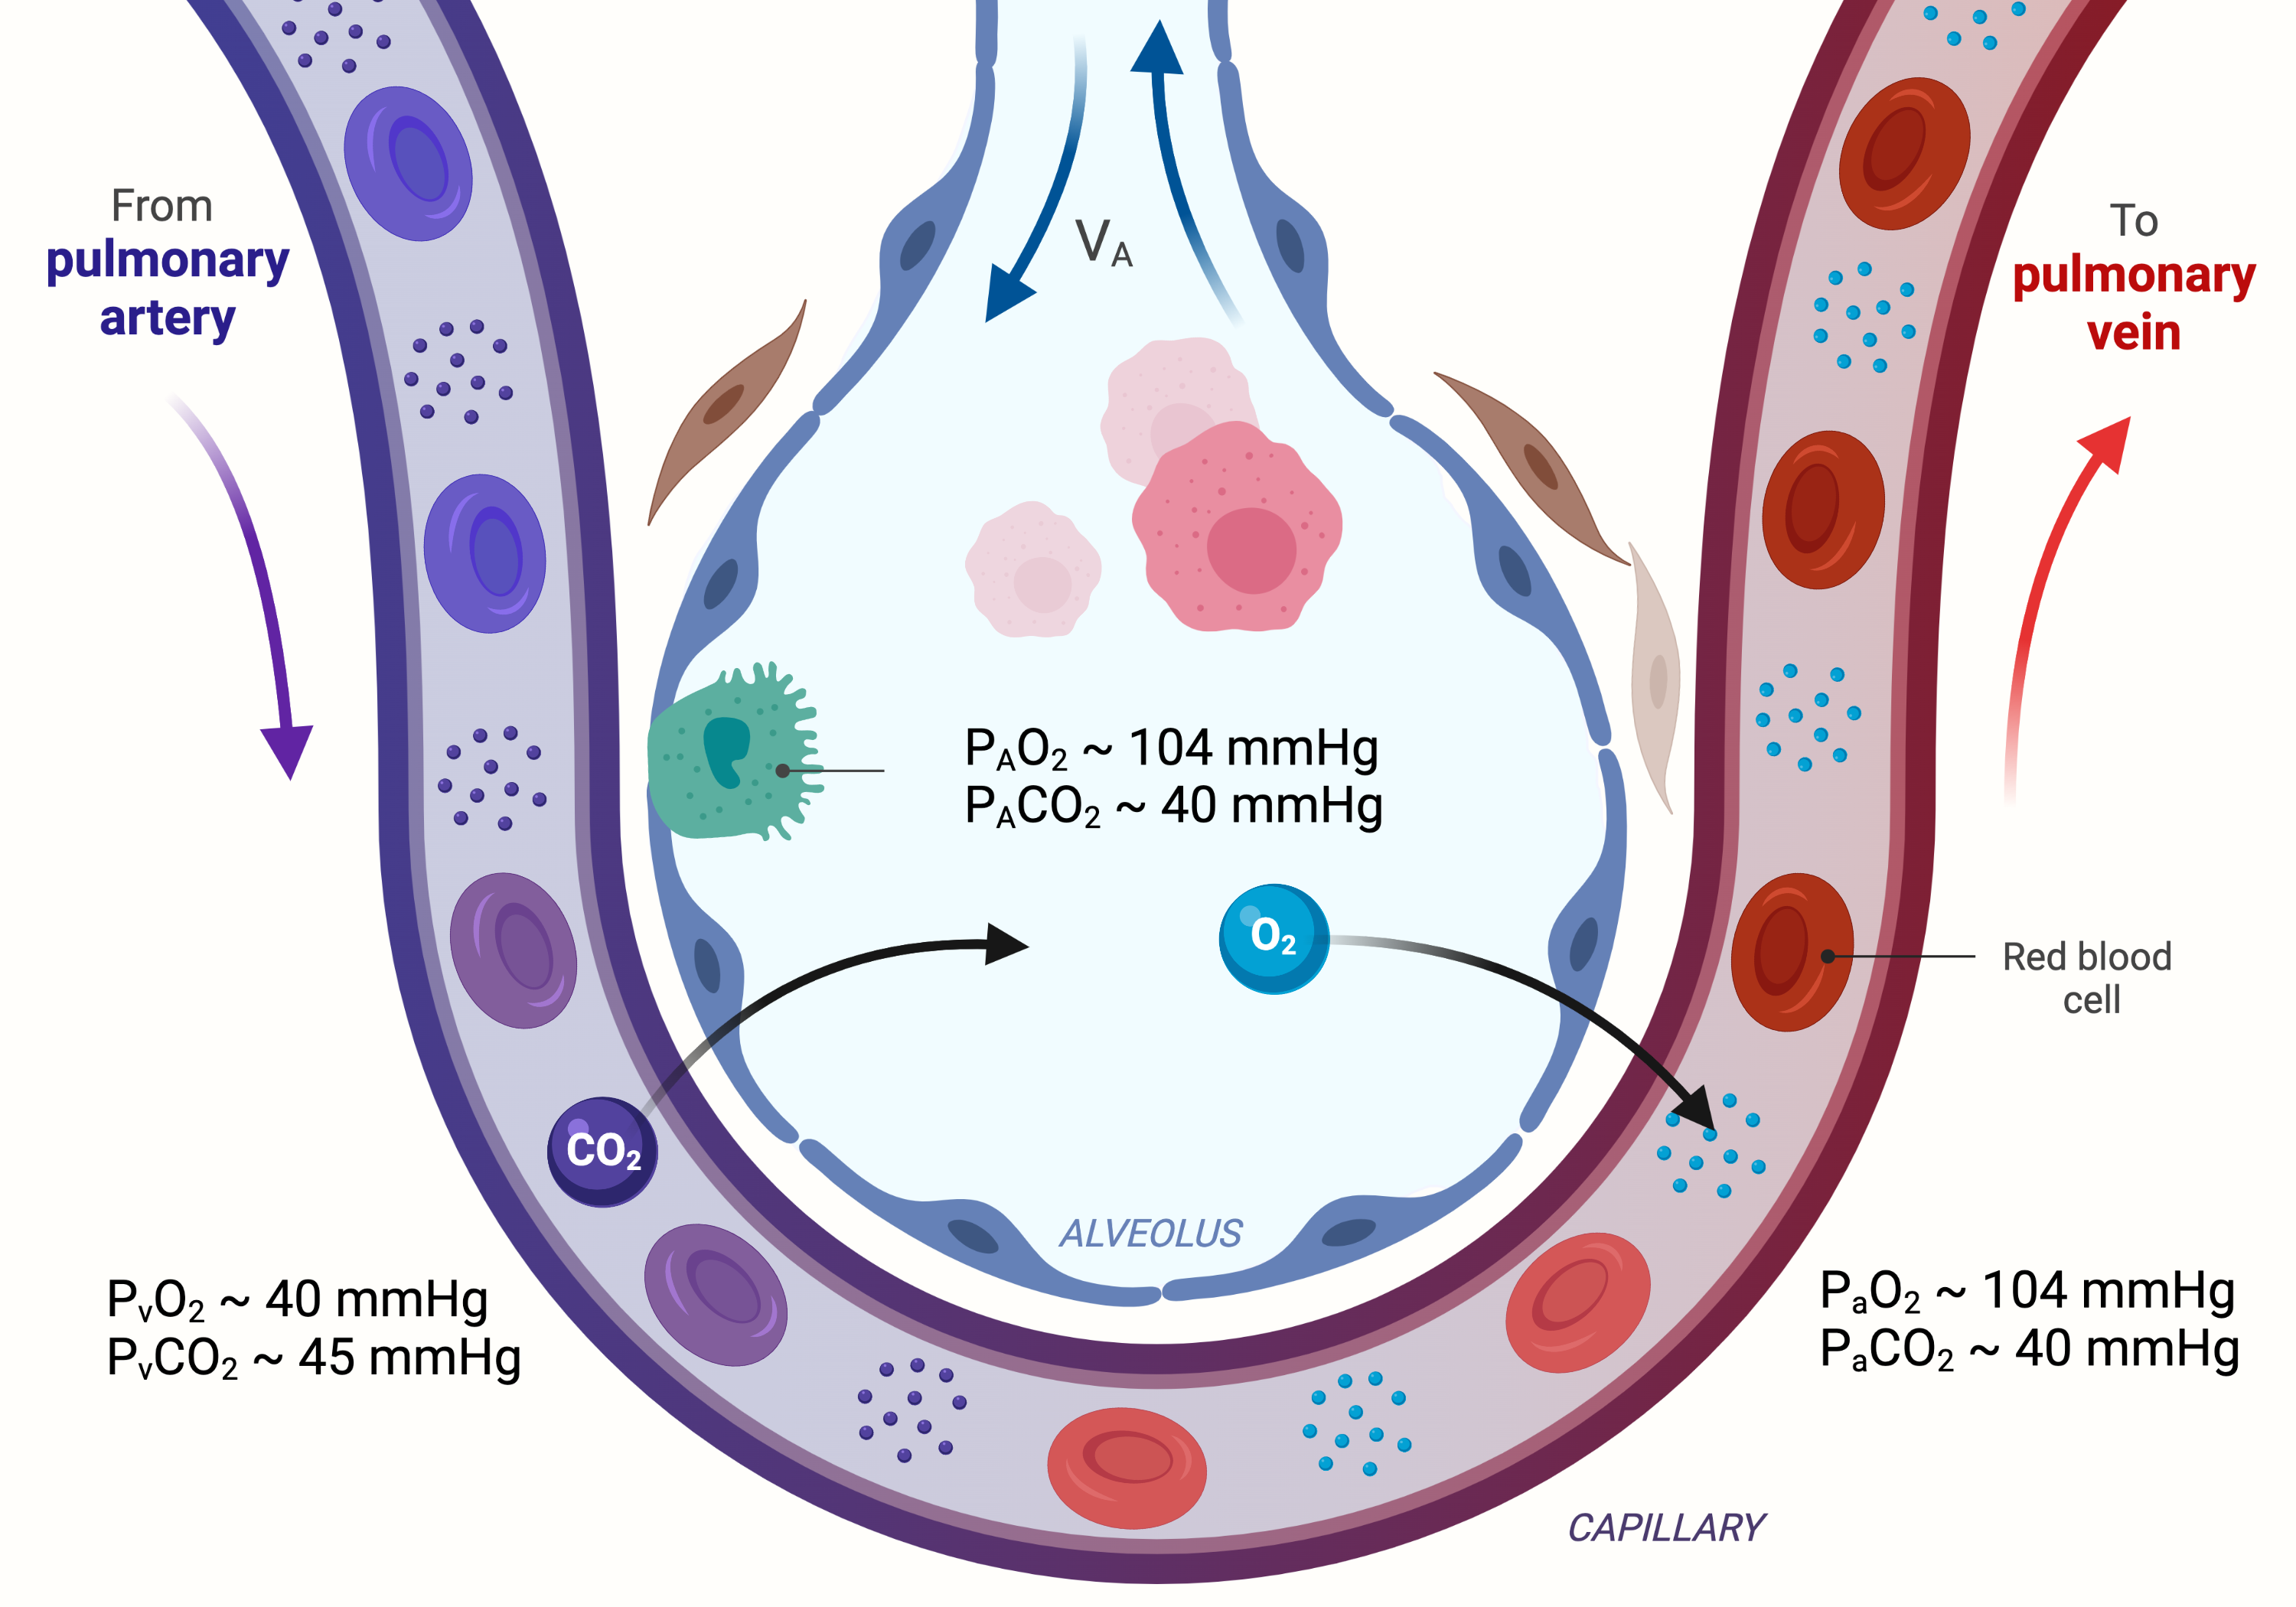
\includegraphics[width=1.0\linewidth]{./figure/alveolar_equilibration.png}
    \caption{Equilibration of Alveolar Diffusion \footnotesize{(Created with BioRender.com)}}
    \label{fig:alveolar_equilibration}
\end{figure}

\paragraph{Atmospheric Limits}

The atmospheric $P_{atm}O_2$ places a limit on how high the alveolar partial pressure ($P_AO_2$) can be and therefore the highest value of $P_AO_2$ and $P_aO_2$. This upper limit means now matter how much someone breathes, there is an upper limit on diffusion of oxygen into the blood. That upper limit is reduced with lower atmospheric $P_{atm}O_2$, which is the case with higher altitude. A hyperbaric (higher pressure) chamber increases $P_{atm}O_2$, and subsequently $P_AO_2$, and $P_aO_2$. 

\paragraph{Supplemental $O_2$}
The use of supplemental $O_2$ changes the $P_AO_2$ and $P_aO_2$ by increasing the $F_iO_2$. Since $PO_2 = F_iO_2 \times Pressure$, then if $F_iO_2$ is 0.4 at sea level the $P_{atm}O_2 = 0.21 \times 760 = 304 mmHg$, and the $P_AO_2 \approx 200 mmHg$. Supplemental $O_2$ is utilized when there are impairments in alveolar respiration or alveolar ventilation. The goal is to treat hypoxemia by improving the partial pressure gradient of $O_2$ in ventilated alveoli to make up for problems in alveoli that otherwise limit diffusion (poor circulation, increased diffusion membrane thickness, decreased diffusion surface area, or poor ventilation). 

% The influence of reduced atmospheric pressure on inspired oxygen is calculated at the effective oxygen percentage ($E_iO_2$). At sea level the $E_iO_2$ is the same as the fraction of inspired oxygen ($F_iO_2$)  and is 0.2099 (usually rounded to 0.21) or 21\%. At the top of Mount Washington (6288 feet), the $E_iO_2 \approx 0.162$. At the top of Mount Everest (29,029 feet), the $E_iO_2 \approx 0.069$. Studies have confirmed that at altitudes higher than 26,000 feet ($\approx$ 8,000 meters) that the $E_iO_2$ of $\approx 0.078$ is not sustainable to life. Practically this means that above that altitude, or below that $E_iO_2$, the body has enough hypoxia that it cannot absorb nutrients or perform vital functions and it starts to shut down. This does not mean sudden death. But it does mean eventual death since the body cannot recover from fatigue, so it does not have the ability to perform the required work:rest cycles for life.

\subsection{Alveolar $CO_2$ Diffusion}

A ventilated alveoli at sea level will have a partial pressure of carbon dioxide ($P_ACO_2$) of approximately 40 $mmHg$. The $PCO_2$ drops dramatically from the arterial blood to the atmosphere ($P_{atm}CO_2 \approx 0.3 mmHg$). The full equilibration of blood so that the $P_aCO_2 = P_ACO_2$ requires alveoli with normal membrane thickness and surface area in contact with capillaries, and normal capillary membranes (See Figure \ref{fig:alveolar_equilibration}). During equilibration of $CO_2$ the processes discussed in the section on $CO_2$ transport in the blood in reverse to release $CO_2$ from the blood (See Figure \ref{fig:co2_transport}). 

\paragraph{Atmospheric Limits}

The atmospheric $PCO_2$ places a very low limit on the alveolar partial pressure ($P_ACO_2$)and therefore there is a very low limit for $P_aCO_2$. The lack of a limit means high alveolar ventilation ($V_A$) can greatly reduce the $P_aCO_2$. The situations of hyperventilation (lower than normal $P_a_CO_2$), and hypoventilation (higher than normal $P_aCO_2$) are discussed in Chapter \ref{chp:alveolar_oxygen}. 

\paragraph{Intentional Hyperventilation}
A popular set of breathing exercises (Wim Hof breathing) make use of hyperventilation to promote reduced $P_aCO_2$ which directly alters blood flow and enables temporary (intermittent) hypoxemia which can be a trigger for intermittent hypoxia intervention. Similarly, deep divers or anyone attempting to promote prolonged breath hold, make use of hyperventilation to lower $P_ACO_2$ to delay the chemoreceptor drive to breath. These topics are covered more completely in the section on ventilatory regulation in the next chapter.

\subsection{$P_aCO_2$ and Brain Blood Flow}

Two mechanisms control brain blood flow by changing blood vessel radius: autoregulation maintains flow in the face of pressure changes, and brain metabolism adjusts flow to meet metabolic requirements. Brain blood vessel reactivity to $P_aCO_2$ is an important component flow adjusting to metabolic requirements. Below a threshold ($P_aCO_2 \approx 36 mmHg$), blood pressure is unchanged, but blood flow increases in response to increased $P_aCO_2$, and decreases in response to decreased $P_aCO_2$. Above the threshold ($P_aCO_2 \approx 36 mmHg$), both blood flow and pressure increase in response to increased $P_aCO_2$, and decrease in response to decreased $P_aCO_2$ \cite{battisti-charbonney_cerebrovascular_2011}. This relationship provides an explanation for lightheadedness during hyperventilation (reduced $P_aCO_2$), and signs and symptoms attributed to hyperventilation (or over breathing) syndrome \cite{courtney_investigating_2008}.

\section{Practice Connections}

\subsection{Arterial Blood Gases}

Arterial Blood Gases (ABGs) are measured from a sample of arterial blood and provide information on the arterial (plasma) partial pressure of $O_2$ and $CO_2$, the arterial blood pH, and the arterial blood bicarbonate ($HCO_3^-$). There are several standards for reporting these values in tabular form. A common convention and normal values are depicted in Table \ref{table:ABGs}

\begin{table}[h!]
\centering
\begin{tabular}{||c|c|c|c||} 
 \hline
 $P_aO_2$ & $P_aCO_2$ & pH & $HCO_3^-$ \\ [0.5ex] 
 \hline
 95-100 $mmHg$ & 35-45 $mmHg$ & 7.35-7.45 & 22-26 $mmol/L$ \\ [1ex] 
 \hline
\end{tabular}
\caption{Normal Ranges of the Arterial Blood Gases}
\label{table:ABGs}
\end{table}

ABGs are extremely valuable measurements for the examination of respiration impairments. Some impairments reduce the $P_aO_2$ (hypoxemia) but do not impact the $P_aCO_2$ and therefore do not create acid base imbalance. Whereas other impairments reduce $P_aO_2$ and increase $P_aCO_2$ (hypercarbia, also known as hypercapnea) and therefore create acid base imbalances (respiratory acidosis).

\subsection{Acid - Base Balance \& Disorders}

Acid base balance is when pH is at it's normal blood level of 7.35-7.45. Acid base balance is maintained due to buffering capacity in both ICF and ECF. The ECF buffering capacity of blood is related to renal functin (long term) and respiration (short term). Disorders of acid base balance are classified as acidosis when pH is below 7.35, and alkalosis when pH is above 7.45. There are two general causes of imbalances, respiratory (due to altered $P_aCO_2$), or metabolic (primarily renal) due to altered $HCO_3^-$. The four possible situations are:
\vspace{3mm}
\begin{itemize}
    \item Respiratory Acidosis: Decreased pH due to elevated $P_aCO_2$
    \item Respiratory Alkalosis: Increased pH due to decreased $P_aCO_2$
    \item Metabolic Acidosis: Decreased pH due to decreased $HCO_3^-$
    \item Metabolic Alkalosis: Increased pH due to increased $HCO_3^-$
\end{itemize}
\vspace{3mm}

Respiratory and renal mechanisms can compensate for acid base disturbances created by the other system. Respiratory compensation refers to the use of respiratory adjustments to $P_aCO_2$ to compensate (normalize, but not completely, pH) when there is a metabolic disturbance. Renal compensation refers to the use of renal clearance adjustments to $HCO_3^-$ and $H^+$ to compensate (normalize, but not completely, pH) when there is a respiratory disturbance. Respiratory compensation is rapid since it simply involves changing breathing rate and depth (ventilation), it can occur in seconds to minutes. Renal compensation involves renal clearance and possibly production of more $HCO_3^-$, so it takes hours to days, depending on what is required, GFR, and urine output (which depends on fluid intake).

\subsubsection{Interpretation of ABGs to Evaluate Acid Base Balance}

Figure \ref{fig:ABGs} provides a decision tree for the evaluation of acid base balance. The process starts with an assessment of the pH. Since compensation can return pH close to the normal of 7.4 (and therefore within the normal range of 7.35-7.45) the process considers the range of pH but decisions of acidosis and alkalosis are initially based on whether pH is below or above 7.4. The decision tree starts with the claim that there is an imbalance even if pH is within the range of 7.35-7.45, so the interpretative process does not simply stop if pH is within the normal range due to compensation.


\begin{figure}[!h]
    \centering
    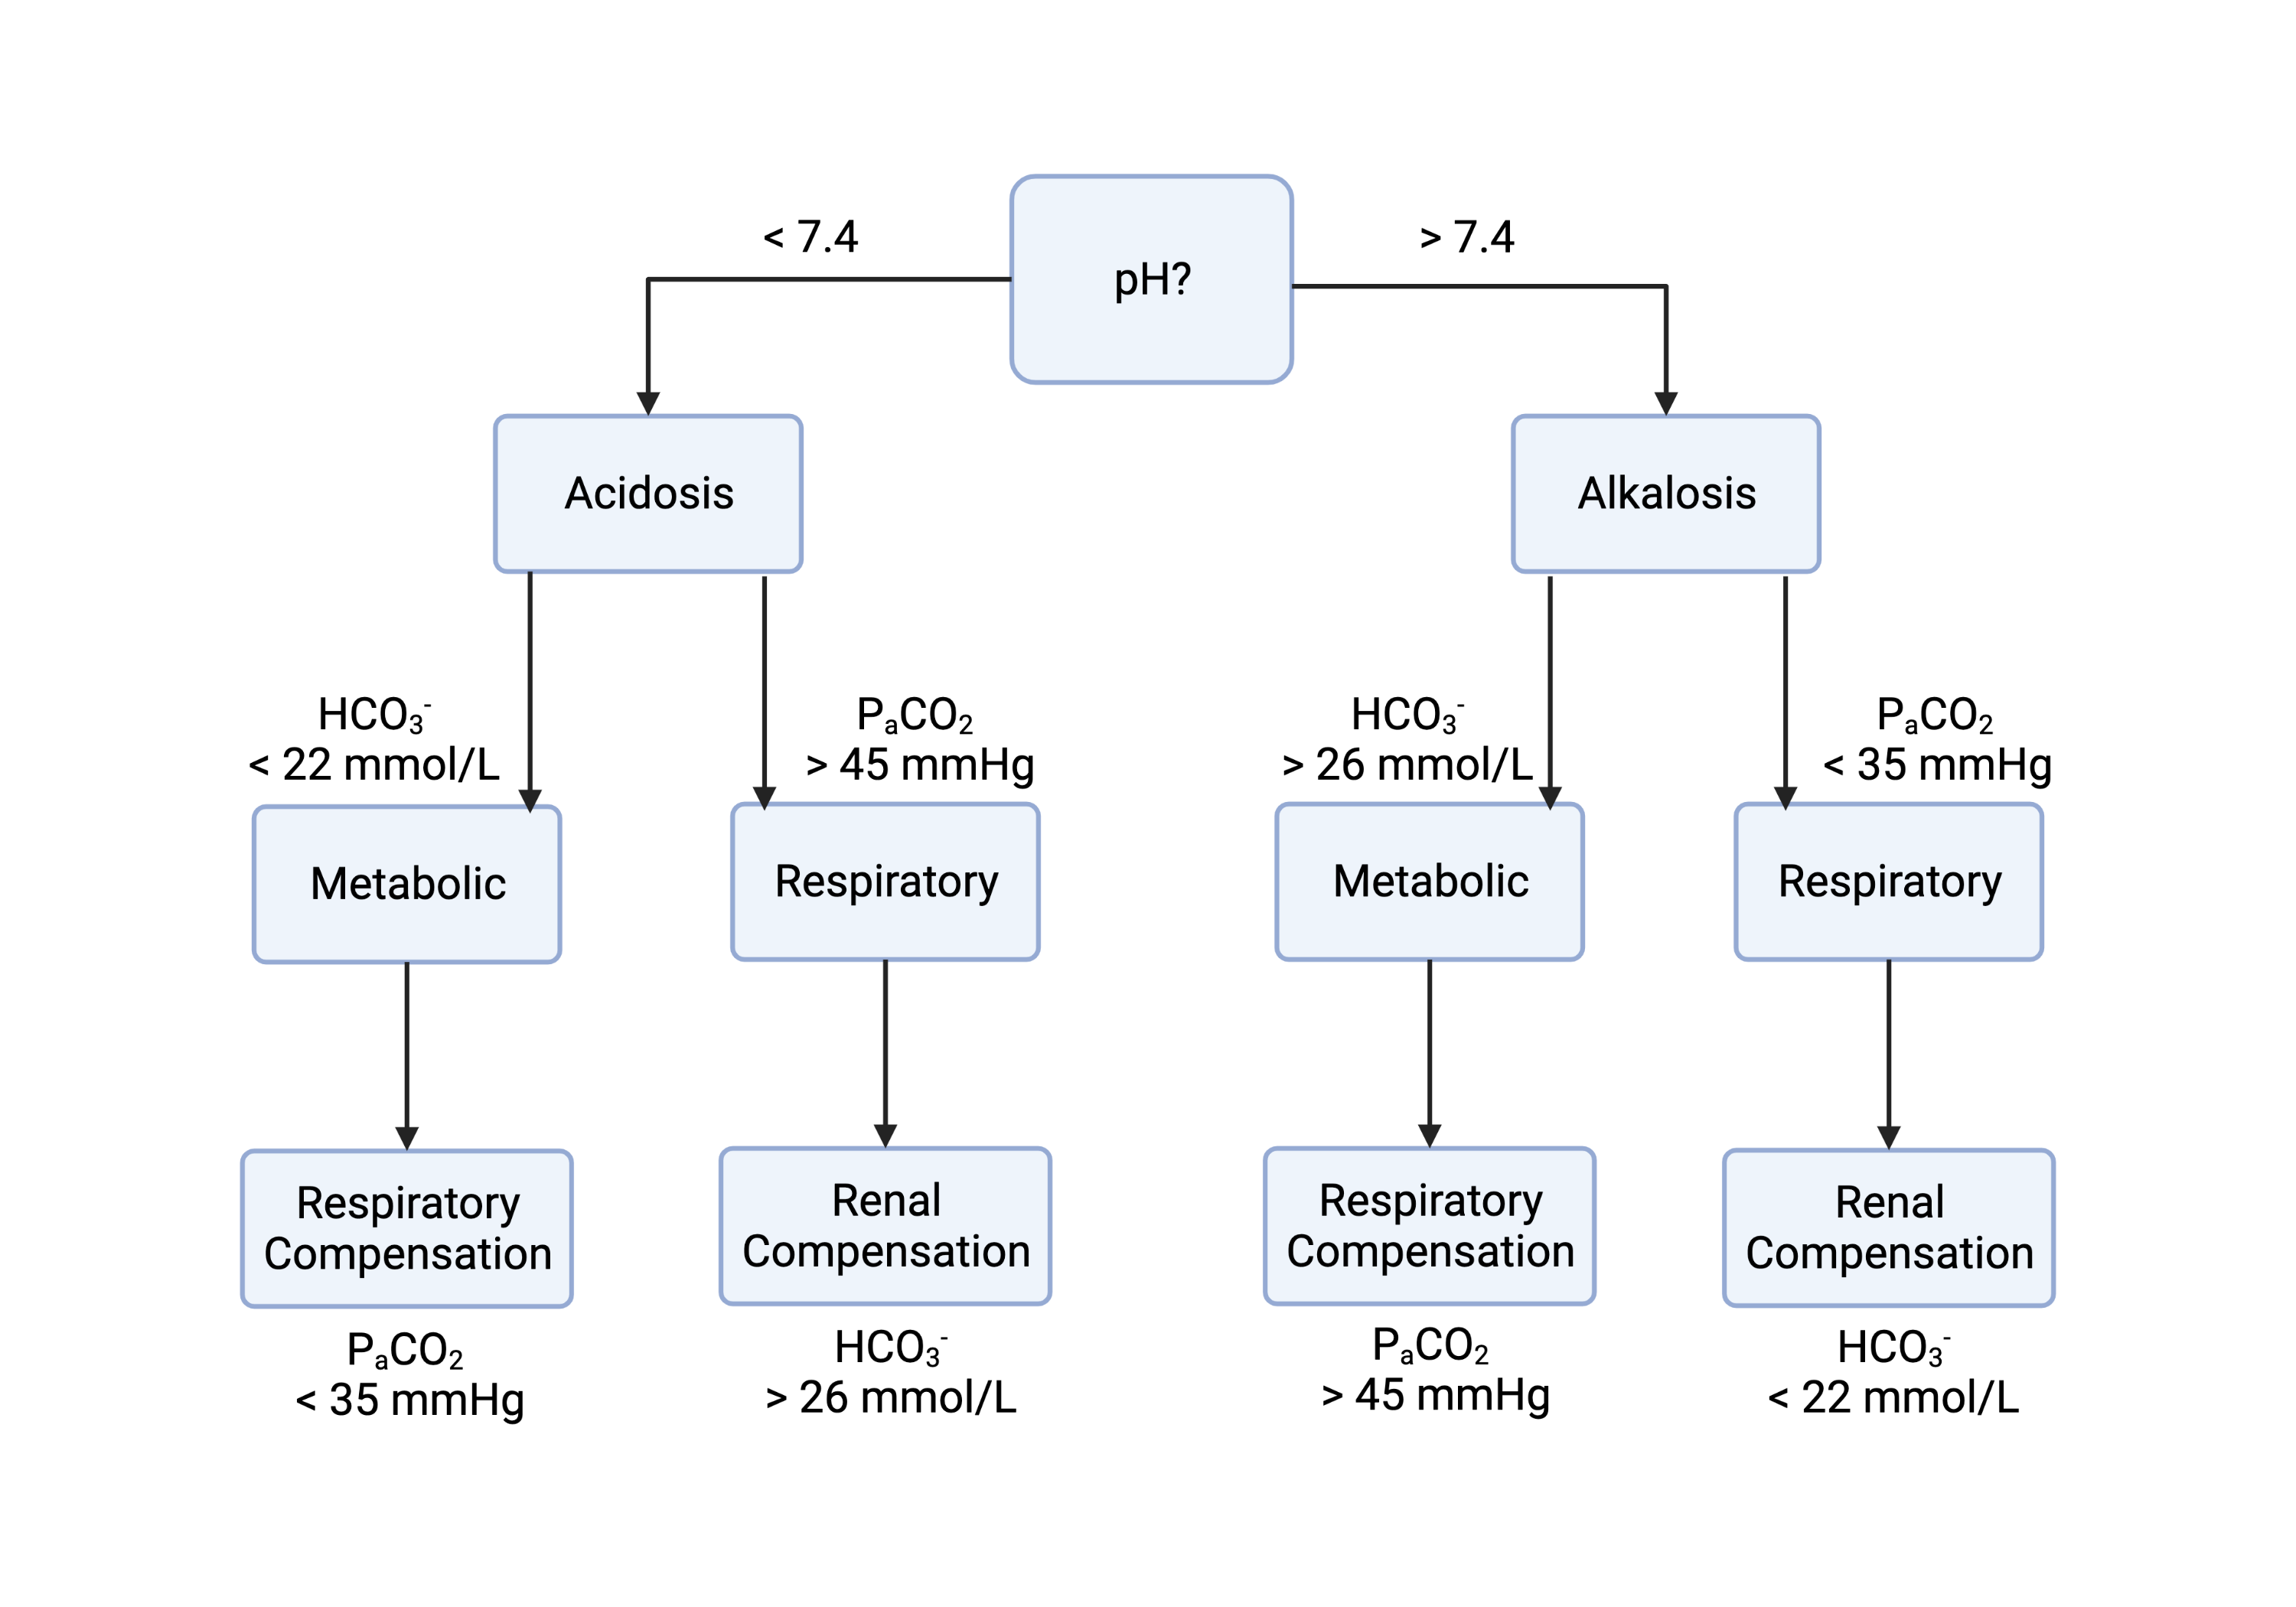
\includegraphics[width=1.0\linewidth]{./figure/ABGs.png}
    \caption{Interpretation of ABGs to Evaluate Acid Base Balance}
    \label{fig:ABGs}
\end{figure}

Individuals with COPD (emphysema and/or chronic bronchitis are the primary causes) tend to have respiration impairments that result in respiratory acidosis due to elevated $P_aCO_2$. Interpretation of ABGs can evaluate whether the current status of a patient is acute or chronic. If a patient has respiratory acidosis that is not compensated then the patient is having an acute exacerbation of their chronic respiration impairment. However, if the respiratory acidosis is compensated then this degree of respiratory acidosis has had sometime for renal compensation to occur. It may still be relatively new for the patient, but since renal compensation can take days, it is not acute in that sense that is is unlikely to be new at the time of measurement.\footnotemark\footnotetext{Need to consider "acute" vs. "chronic" with regard to respiration impairments since many problems can be acute but still be a day old. The best way to know whether someone's respiration impairment is worsened is to compare to previous ABG measurements, ideally those taken when not in distress.}

\subsection{Pulmonary Function Testing - DLCO}
DLCO is a pulmonary function test that evaluates the diffusion capacity of the lung for carbon monoxide ($CO$)). It is used to evaluate the extent that $O_2$ diffuses across the alveoli-capillary membrane into the capillary blood impacting the $P_aO_2$. The test involves measuring the partial pressure difference between inspired and expired $CO$. It relies on the strong affinity and large absorption capacity of red blood cells for carbon monoxide and demonstrates gas uptake by the capillary blood. DLCO is also affected by the HgB, carboxyhemoglobin, age and sex. DLCO is measured in $ml/min/kPa$ ($kPa$ as an SI unit of pressure, the kilopascal). However, DLCO is usually reported as a percent of predicted value based on age and sex. Values between 80-120\% predicted are generally accepted as normal. Values below 80\% indicate possible limitations to $O_2$ diffusion in the lung. With a low DLCO it is less likely that capillary blood will equilibrate with $P_AO_2$ while in the alveolar capillary, and is therefore more likely that $P_aO_2$ will be reduced.
DLCO may be reduced in individuals with conditions that impact the thickness or surface area of alveoli (Equation \ref{diffusion}) such as emphysema, pulmonary fibrosis, or pulmonary hypertension.
DLCO helps with examination of whether someone has a respiration impairment and the risk that they will have hypoxemia at rest, or become hypoxemic with exertion.

\subsection{Pulsed Oximetry}

Pulsed oximetry indirectly monitors the $O_2$ saturation of arterial blood ($S_pO_2$) as opposed to a measurement directly from arterial blood ($S_aO_2$). A pulsed oximetry device is commonly referred to as an oximeter, or more colloquially a "pulse ox". 
Oximeters use an electronic processor and two small light-emitting diodes (LEDs) facing a photodiode through a translucent part of the skin, such as a fingertip or earlobe. Each LED emits a different wavelength of light. Absorption of light at these wavelengths differs significantly between $O_2$-HgB and HgB. The amount of light not absorbed from each LED is measured, and separate normalized signals are produced for each wavelength. These signals fluctuate in time because the amount of arterial blood that is present increases (literally pulses) with each heartbeat. The signals are used to calculate an estimate of $S_aO_2$ known as $S_pO_2$. Most units are accurate within 2.5\% down to approximately 70\% saturation. The signals also reflect the volume of pulsatile capillary flow (photoplethysmogram (PPG)) that pulses with left ventricular systole and can therefore also be used to determine pulse rate (as an estimate of heart rate), and indices related to blood flow volume and timing.

Poor blood flow to the extremity may cause erroneously low readings which can be as simple as a cold limb, or vasoconstriction (so not all low readings are low). There are no known causes of erroneously high readings (so normal / high readings tend to be accurate).\footnotemark\footnotetext{This means that as an indicator of hypoxemia, oximetry has more false positives and limited false negatives. Such a diagnostic accuracy measurement is said to have low specificity and high sensitivity and are better for ruling out a situation than they are for ruling in a situation. For example, if $S_pO_2$ is normal then we are confident it is normal so we feel confident we have ruled out hypoxemia. If $S_pO_2$ is less than 89\% we have less confidence about hypoxemia because there is a risk of a false positive, so we have less confidence to rule in hypoxemia.} Other problems can include incorrect sensor application (such as not placing the LEDs on the thinner skin surface area); highly calloused skin; movement; finger nail polish; or higher skin pigmentation. Oximeters that include a PPG waveform are usually more expensive but allow an assessment of sensor accuracy by verification that the sensor is producing a steady pulse waveform. In the absence of a PPG waveform another approach to confirm accuracy is to verify the pulse rate estimate from the oximeter is the same as the radial pulse.

$S_pO_2$ helps to examine whether someone has hypoxemia at the time of measurement. Since it is easily measured, it provides continuous information about hypoxemia. For example, in someone with COPD that has a reduced DLCO but is not hypoxemic at rest, using an oximeter to monitor the $S_pO_2$ allows the clinician to know the point in time that the patient became hypoxemic, either due to exertion with exercise, ADLs, or position changes.

\section{Summary}

The mass balance of $O_2$ and $CO_2$ requires the diffusion of these gases at several points along what is a long chain of intake (for $O_2$) and output (for $CO_2$). Cellular and internal respiration, blood transport, and external respiration are all necessary and important steps in this system wide gas exchange. Understanding these steps and the factors that influence the steps are important for understanding the normal response to increased muscle need for $O_2$, and situations that include impairments at any point along the pathway for $O_2$. Clinical approaches exist to evaluate the current status of respiration (ABGs and oximetry). ABGs provide more information but require arterial blood sampling. Oximetry provides less information, but is easily obtained for continuous monitoring. DLCO provides an evaluation of the risk of hypoxemia. 


\subsection{Next Step}

This chapter presents an incomplete story of overall pulmonary support for the mass balance of $O_2$ and $CO_2$. It leaves off with alveolar respiration, and only considers alveolar respiration at one alveolus. In the next chapter we consider ventilation (breathing) mechanics and the process of drawing air into and out of the alveoli. Without continuous alveolar ventilation ($V_A$) there is no alveolar respiration; and without ventilation ($V_e$), there is no $V_A$. We also consider the importance of the distribution of $V_e$ throughout the lungs that results in regional differences in $V_A$, and the distribution of pulmonary perfusion ($\dot{Q}$). Alveolar respiration cannot occur unless there is $V_A$ matched with capillary blood flow (perfusion). 

%The regulation of blood $O_2$ and $CO_2$ includes monitoring these values with chemoreceptors, but the efferent (action) side of these regulatory pathways include variations in ventilation.

\printbibliography[heading=subbibintoc]